%
% Template Laporan Skripsi/Thesis Universitas Indonesia
%
% @author  Ichlasul Affan, Azhar Kurnia
% @version 2.1.2
%
% Dokumen ini dibuat berdasarkan standar IEEE dalam membuat class untuk
% LaTeX dan konfigurasi LaTeX yang digunakan Fahrurrozi Rahman ketika
% membuat laporan skripsi, yang kemudian diadaptasi oleh Andreas Febrian dan
% Lia Sadita untuk template skripsi tahun 2010.
% Konfigurasi template sebelumnya telah disesuaikan dengan
% aturan penulisan thesis yang dikeluarkan UI pada tahun 2017.
%

%
% Tipe dokumen adalah report dengan satu kolom.
%
\documentclass[12pt, a4paper, onecolumn, twoside, final]{report}
\raggedbottom

% Load konfigurasi LaTeX untuk tipe laporan thesis
\usepackage{_internals/uithesis}
%

\usepackage[]{minted}
\usepackage{tcolorbox}
\usepackage{etoolbox}
\usepackage[T1]{fontenc}
\usepackage{inconsolata}

\usepackage{titlesec}
\usepackage{natbib}
\usepackage{multirow}
\titleformat{\section}
  {\normalfont\fontsize{12}{15}\bfseries}{\thesection}{0.5em}{}
\titleformat{\subsection}
  {\normalfont\fontsize{12}{15}\bfseries}{\thesubsection}{0.5em}{}
\titleformat{\subsubsection}
  {\normalfont\fontsize{12}{15}\bfseries}{\thesubsubsection}{0.5em}{}

\newcommand{\listmintedcodename}{Daftar Kode Program}
\newlistof{mintedcode}{mcode}{\listmintedcodename}

% (Bahasa, file, caption)
\newcommand{\mintedcode}[3]{%
    \refstepcounter{mintedcode}
    \begin{tcolorbox}[boxrule=0.5pt,leftrule=0.5pt,arc=0pt,auto outer arc]
        \setstretch{0.9}
        \inputminted[]{#1}{#2}
    \end{tcolorbox}
    \begin{@empty}
        \setlength\topsep{0pt}
        \setlength\parskip{0pt}
        \begin{center}
            \par\noindent\textbf{Kode \thechapter.\themintedcode. #3}
        \end{center}
    \end{@empty}
    \addcontentsline{mcode}{mintedcode}
    {\protect\numberline{\thechapter.\themintedcode}#3}\par
}

% Load konfigurasi khusus untuk laporan yang sedang dibuat
%-----------------------------------------------------------------------------%
% Informasi Mengenai Dokumen
%-----------------------------------------------------------------------------%
%

% Judul laporan.
\def\judul{PeerToCP: Editor Kode dan \textit{Shared Terminal} Kolaboratif dalam Waktu Nyata Berbasis {WebRTC}}
%
% Tulis kembali judul laporan, kali ini akan diubah menjadi huruf kapital
\Var{\Judul}{PeerToCP: Editor Kode dan \textit{Shared Terminal} Kolaboratif dalam Waktu Nyata Berbasis {WebRTC}}
%
% Tulis kembali judul laporan namun dengan bahasa Ingris
\def\judulInggris{PeerToCP: WebRTC Based Real-Time Collaborative Code Editor and Shared Terminal}

% Tipe laporan, dapat berisi: Laporan Kerja Praktik, Skripsi, Tugas Akhir, Thesis, atau Disertasi
\def\type{Skripsi}
%
% Jenjang studi, dapat berisi: Diploma, Sarjana, Magister, atau Doktor
\def\jenjang{Sarjana}
%
% Tulis kembali tipe laporan, kali ini akan diubah menjadi huruf kapital
\Var{\Type}{Skripsi}
%
% Tulis nama penulis
\def\penulis{Hocky Yudhiono}
%
% Tulis kembali nama penulis, kali ini akan diubah menjadi huruf kapital
\Var{\Penulis}{Hocky Yudhiono}
%
% Tulis NPM penulis
\def\npm{1906285604}
%
% Tuliskan Fakultas dimana penulis berada
\Var{\Fakultas}{Ilmu Komputer}
\def\fakultas{Ilmu Komputer}
%
% Tuliskan Program Studi yang diambil penulis
\Var{\Program}{Ilmu Komputer}
\def\program{Ilmu Komputer}
% Program Studi dalam bahasa inggris
\def\studyProgram{Computer Science}
%
% Tuliskan tahun publikasi laporan
\Var{\bulanTahun}{Desember 2022}
%
% Tuliskan gelar yang akan diperoleh dengan menyerahkan laporan ini
\def\gelar{Sarjana Ilmu Komputer}
%
% Tuliskan tanggal pengesahan laporan, waktu dimana laporan diserahkan ke
% penguji/sekretariat
\def\tanggalSiapSidang{20 November 2022}
%
% Tuliskan tanggal keputusan sidang dikeluarkan dan penulis dinyatakan
% lulus/tidak lulus
\def\tanggalLulus{1 Desember 2022}
%
% Tuliskan pembimbing
\def\pembimbingSatu{Muhammad Hafizhuddin Hilman S.Kom., M.Kom., Ph.D.}
% S1 s.d. S3: Kosongkan jika tidak ada pembimbing kedua
\def\pembimbingDua{}
% S2 & S3: Kosongkan jika tidak ada pembimbing ketiga
\def\pembimbingTiga{}
%
% Tuliskan penguji
\def\pengujiSatu{Penguji Pertama Anda}
\def\pengujiDua{Penguji Kedua Anda}
% Kosongkan jika tidak ada penguji ketiga (umumnya penguji ketiga hanya ada untuk S2)
\def\pengujiTiga{}
% Kosongkan jika tidak ada penguji keempat, kelima, atau keenam (umumnya penguji > 3 hanya ada untuk S3)
\def\pengujiEmpat{}
\def\pengujiLima{}
\def\pengujiEnam{}

%-----------------------------------------------------------------------------%
% Judul Setiap Bab
%-----------------------------------------------------------------------------%
%
% Berikut ada judul-judul setiap bab.
% Silahkan diubah sesuai dengan kebutuhan.
%
\Var{\kataPengantar}{Kata Pengantar}
\Var{\babSatu}{Pendahuluan}
\Var{\babDua}{Tinjauan Pustaka}
\Var{\babTiga}{Metodologi Penelitian}
\Var{\babEmpat}{Desain dan Implementasi}
\Var{\babLima}{Hasil dan Pembahasan}
\Var{\kesimpulan}{Penutup}

% Daftar pemenggalan suku kata dan istilah dalam LaTeX
%
% Hyphenation untuk Indonesia
%
% @author  Andreas Febrian
% @version 2.1.2
% @edit by Ichlasul Affan, Muhammad Aulia Adil Murtito
%
% Tambahkan cara pemenggalan kata-kata yang salah dipenggal secara otomatis
% oleh LaTeX. Jika kata tersebut dapat dipenggal dengan benar, maka tidak
% perlu ditambahkan dalam berkas ini. Tanda pemenggalan kata menggunakan
% tanda '-'; contoh:
% menarik
%   --> pemenggalan: me-na-rik
%


% Silakan ganti ke bahasa Inggris (\selectlanguage{english}) jika Anda merasa terlalu banyak kata bahasa Inggris yang pemenggalannya tidak benar.
%\selectlanguage{english}


\hyphenation{
    % alphabhet A
    a-na-li-sa a-tur a-tur-an
    a-pli-ka-si a-pli-ka-si-nya
    % alphabhet B
    bab ba-ngun-an
    be-be-ra-pa
    ber-ge-rak
    ber-ke-lan-jut-an
    ber-o-per-ra-si
    ber-pe-nga-ruh
    % alphabhet C
    chan-nel
    con-nec-tiv-i-ty
    ca-ri Com-po-nent-UML
    % alphabhet D
    di-da-pat-kan di-sim-pan di-pim-pin di-tam-bah-kan di-tem-pat-kan de-ngan da-e-rah di-ba-ngun di-gu-na-kan da-pat di-nya-ta-kan
    di-se-mat-kan di-sim-bol-kan di-pi-lih di-li-hat de-fi-ni-si di-de-fi-ni-si-kan di-mo-del-kan di-mi-li-ki di-re-a-li-sa-si-kan di-su-sun
    di-te-rap-kan
    di-se-le-sai-kan
    % alphabhet E
    eks-pli-sit e-ner-gi en-gi-neer en-gi-neer-ing eks-klu-sif ele-men
    es-tab-lish-ment en-vi-ron-ment
    eks-pe-ri-men
    % alphabhet F
    fa-si-li-tas
    % alphabhet G
    ga-bung-an ge-rak ge-ne-ral ge-ne-ra-li-sa-si
    % alphabhet H
    ha-lang-an
    % alphabhet I
    in-fra-struk-tur i-ni-si-a-si
    % alphabhet J
    % alphabhet K
    ko-la-bo-ra-tif
    ke-hi-lang-an
    ke-ter-hu-bung-an
    ku-ning
    kua-li-tas ka-me-ra ke-mung-kin-an ke-se-pa-ham-an
    % alphabhet L
    ling-kung-an
    lo-gi-cal
    % alphabhet M
    ma-na-je-men me-neng-ah meng-a-da-kan me-mo-ni-tor
    me-mer-lu-kan me-mo-del-kan men-de-fi-ni-si-kan meng-ak-ses me-ne-mu-kan
    meng-a-tas-i me-mo-di-fi-ka-si me-mung-kin-kan me-nge-na-i me-ngi-rim-kan meng-i-zin-kan
    meng-u-bah meng-a-dap-ta-si me-nya-ta-kan me-nyim-pan me-res-trik-si mi-cro-ser-vi-ce mi-cro-ser-vi-ces mo-di-fi-ka-si mo-dul mo-dule
    meng-a-tur meng-a-rah-kan mi-lik meng-gu-na-kan me-ne-ri-ma me-nga-la-mi
    me-di-a-stream-track
    me-di-a-stream
    me-mo-ri
    % alphabhet N
    nya-ta non-eks-klu-sif né-de-lec
    % alphabhet O
    o-pe-ra-si or-ga-ni-sa-si
    % alphabhet P
	pe-nye-rap-an
    peer-to-cp
	pe-ngon-trol
    pe-mo-del-an
    pe-ran  pe-ran-an-nya
    pem-ba-ngun-an pre-si-den pe-me-rin-tah pe-mi-li-han prio-ri-tas peng-am-bil-an
    peng-ga-bung-an pe-nga-was-an pe-ngem-bang-an
    pe-nga-ruh pe-nge-lo-la pa-ra-lel-is-me per-hi-tung-an per-ma-sa-lah-an
    pen-ca-ri-an pen-ce-ta-kan peng-struk-tur-an pen-ting pen-ting-nya pe-ngu-ku-ran
    pre-sen-ta-si pe-nyo-co-kan
    % alphabhet Q
    % alphabhet R
    re-pli-ka
    ran-cang-an re-fe-ren-si re-pre-sen-ta-si
    rtc-da-ta-chan-nel
    ru-a-ngan
    % alphabhet S
    sub-bab si-mu-la-si sa-ngat ska-la-bi-li-tas
    stan-dar-di-sa-si sig-nalling
    sa-tu-an
    ser-ver
    sig-nal-ing
    % alphabhet T
    te-ngah
    ter-da-pat
    trans-for-ma-si
    % alphabhet U
    u-ti-li-sa-si
    % alphabhet V
    va-li-da-si va-ri-an va-ri-a-si va-ri-a-bi-li-tas ve-ri-fi-ka-si
    % alphabhet W
    web-rtc
    % alphabhet X
    % alphabhet Y
    % alphabhet Z
    % special
}

% Daftar istilah yang mungkin perlu ditandai
%
% @author  Andreas Febrian
% @version 1.00
%
% Mendaftar seluruh istilah yang mungkin akan perlu dijadikan
% italic atau bold pada setiap kemunculannya dalam dokumen.
%

\var{\license}{\f{Creative Common License 1.0 Generic}}
\var{\bslash}{$\setminus$}


\renewenvironment{newminted}[2]% environment name
{% begin code
 
}%
{% end code
}

% Awal bagian penulisan laporan
\begin{document}
%
% Sampul Laporan
%
% Sampul Laporan

%
% @author  unknown
% @version 1.01
% @edit by Andreas Febrian
%

\begin{titlepage}
    \begin{center}
        \begin{figure}
            \begin{center}
                
\includegraphics[width=2.5cm]{assets/pics/makara_kuning.png}
            \end{center}
        \end{figure}
        \vspace*{0cm}
        \bo{
        	UNIVERSITAS INDONESIA\\
        }

        \vspace*{1.0cm}
        % judul thesis harus dalam 14pt Times New Roman
        \bo{\Judul} \\[1.0cm]

        \vspace*{2.5 cm}
        % harus dalam 14pt Times New Roman
        \bo{\Type}

        \vspace*{3 cm}
        % penulis dan npm
        \bo{\Penulis} \\
        \bo{\npm} \\

        \vspace*{5.0cm}

        % informasi mengenai fakultas dan program studi
        \bo{
        	FAKULTAS \Fakultas\\
        	PROGRAM STUDI \Program \\
        	DEPOK \\
        	\bulanTahun
        }
    \end{center}
\end{titlepage}

\forceclearchapter

%
% Gunakan penomeran romawi
\pagenumbering{roman}
%
% Menghilangkan penebalan pada huruf-huruf table of content
% dari halaman judul hingga daftar lampiran
\disableboldchapterintoc
%
% load halaman judul dalam
\addChapter{HALAMAN JUDUL}
%
% Halaman Judul Laporan
%
% @author  unknown
% @version 1.01
% @edit by Andreas Febrian
%

\begin{titlepage}
    \begin{center}\begin{figure}
            \begin{center}
                
\includegraphics[width=2.5cm]{assets/pics/makara.png}
            \end{center}
        \end{figure}
        \vspace*{0cm}
        \bo{
        	UNIVERSITAS INDONESIA\\
        }

        \vspace*{1.0cm}
        % judul thesis harus dalam 14pt Times New Roman
        \bo{\Judul} \\[1.0cm]

        \vspace*{2.5 cm}
        % harus dalam 14pt Times New Roman
        \bo{\Type} \\
        % keterangan prasyarat
        \bo{Diajukan sebagai salah satu syarat untuk memperoleh gelar \\
        \gelar}\\

        \vspace*{3 cm}
        % penulis dan npm
        \bo{\Penulis} \\
        \bo{\npm} \\

        \vspace*{4.0cm}

        % informasi mengenai fakultas dan program studi
        \bo{
        	FAKULTAS \Fakultas\\
        	PROGRAM STUDI \Program \\
        	DEPOK \\
        	\bulanTahun
        }
    \end{center}
\end{titlepage}

\forceclearchapter

%
% load halaman orisinalitas

% Menghilangkan penomoran
\pagenumbering{gobble}

\strcompare{Laporan Kerja Praktik}{\type}{}
{
	%
% Halaman Orisinalitas
%
% @author  Andreas Febrian
% @version 2.1.2
% @edit by Muhammad Aulia Adil Murtito
%

\chapter*{\uppercase{Halaman Pernyataan Orisinalitas}}
\thispagestyle{empty}
\vspace*{2cm}

% Untuk input gambar tanda tangan, silahkan sesuaikan xshift, yshift, dan width dengan gambar tanda tangan Anda
%\begin{tikzpicture}[remember picture,overlay,shift={(current page.north east)}]
%\node[anchor=north east,xshift=-8.5cm,yshift=-14.2cm]{\includegraphics[width=3cm]{assets/pics/tanda_tangan_wikipedia.png}};
%\end{tikzpicture}

\begin{center}
	\bo{\type~ini adalah hasil karya saya sendiri, \\
	dan semua sumber baik yang dikutip maupun dirujuk \\
	telah saya nyatakan dengan benar.} \\
	\vspace*{2.6cm}

	\begin{tabular}{l c l}
	\bo{Nama} & : & \bo{\penulis} \\
	\bo{NPM} & : & \bo{\npm} \\
	\bo{Tanda Tangan} & : & \\
	& & \\
	& & \\
	\bo{Tanggal} & : & \bo{\tanggalSiapSidang} \\
	\end{tabular}
\end{center}

\newpage

	\forceclearchapter
}

% Memunculkan penomoran kembali
\pagenumbering{roman}

%
% setelah bagian ini, halaman dihitung sebagai halaman ke 2
\setcounter{page}{2}

%
% Lembar Penegesahan
\strcompare{Laporan Kerja Praktik}{\type}
{
	% Lembar Pengesahan Kerja Praktik dari LaTeX
	\addChapter{LEMBAR PERSETUJUAN DOSEN KERJA PRAKTIK}
	%
% Halaman Pengesahan Laporan Kerja Praktik
%
% @author  Andreas Febrian, Andre Tampubolon
% @version 2.1.2
% @edit by Ichlasul Affan
%

\chapter*{HALAMAN PERSETUJUAN DOSEN KERJA PRAKTIK}
\thispagestyle{empty}
\vspace*{0.4cm}
\noindent

\noindent
\begin{tabular}{ll p{9cm}}
	\multicolumn{3}{l}{\type~ini diajukan oleh:}  \\
	Nama&: & \penulis \\
	NPM&: & \npm \\
	Program Studi&: & \program \\
	Judul Kerja Praktik&: & \judul \\
\end{tabular} \\

\vspace*{1.0cm}

\noindent \bo{Telah berhasil diselesaikan laporan kerja praktik untuk
Fakultas \fakultas~dan dipresentasikan hasil kerja praktiknya sebagai
persyaratan yang harus dipenuhi dalam mata kuliah Kerja Praktik.}\\[0.2cm]

\begin{center}
	DOSEN MATA KULIAH KERJA PRAKTIK\\[2cm]
\end{center}

\begin{center}
	\underline{\pembimbingSatu}\\[0.1cm]
\end{center}

\vspace*{2.0cm}

\begin{tabular}{ll l}
	Ditetapkan di&: & Depok\\
	Tanggal&: & \tanggalLulus \\
\end{tabular}

\newpage

	\forceclearchapter
}
{
	\addChapter{LEMBAR PENGESAHAN}
	% Gunakan salah satu (comment atau hapus kode yang tidak perlu):
	% Lembar Pengesahan Tugas Akhir dari LaTeX
	\strcompare{Doktor}{\jenjang}
	{%
% Halaman Pengesahan Sidang (S3)
%
% @author  Andreas Febrian, Andre Tampubolon
% @version 2.1.2
% @edit by Ichlasul Affan
%

\chapter*{HALAMAN PENGESAHAN}
\thispagestyle{empty}
\vspace*{0.4cm}
\noindent

\noindent
\begin{tabular}{ll p{9cm}}
	\type~ini diajukan oleh&: & \\
	Nama&: & \penulis \\
	NPM&: & \npm \\
	Program Studi&: & \program \\
	Judul \type&: & \judul \\
\end{tabular} \\

\vspace*{1.0cm}

\noindent \bo{Telah berhasil dipertahankan di hadapan Dewan Penguji
dan diterima sebagai bagian persyaratan yang diperlukan untuk
memperoleh gelar Doktor pada Program Studi \program, Fakultas
\fakultas, Universitas Indonesia.}\\[0.2cm]

\begin{center}
	\bo{DEWAN PENGUJI}
\end{center}

\vspace*{0.3cm}

\def\blank{}
\begin{longtable}{l l p{7cm} l }
	\centering
	& & & \\
	Promotor&: & \pembimbingSatu & (\hspace*{3.0cm}) \\
	\ifx\blank\pembimbingDua
    \else
        & & & \\
    	Kopromotor&: & \pembimbingDua & (\hspace*{3.0cm}) \\
    \fi
    \ifx\blank\pembimbingTiga
    \else
        & & & \\
    	&: & \pembimbingTiga & (\hspace*{3.0cm}) \\
    \fi
	& & & \\
	Tim Penguji&: & \pengujiSatu~(Ketua) & (\hspace*{3.0cm}) \\
	& & & \\
	&: & \pengujiDua~(Anggota) & (\hspace*{3.0cm}) \\
	\ifx\blank\pengujiTiga
    \else
        & & & \\
    	&: & \pengujiTiga~(Anggota) & (\hspace*{3.0cm}) \\
    \fi
	\ifx\blank\pengujiEmpat
	\else
		& & & \\
		&: & \pengujiEmpat~(Anggota) & (\hspace*{3.0cm}) \\
	\fi
	\ifx\blank\pengujiLima
	\else
		& & & \\
		&: & \pengujiLima~(Anggota) & (\hspace*{3.0cm}) \\
	\fi
	\ifx\blank\pengujiEnam
	\else
		& & & \\
		&: & \pengujiEnam~(Anggota) & (\hspace*{3.0cm}) \\
	\fi
\end{longtable}

\vspace*{2.0cm}

\begin{tabular}{ll l}
	Ditetapkan di&: & Depok\\
	Tanggal&: & \tanggalLulus \\
\end{tabular}


\newpage
}
	{%
% Halaman Pengesahan Sidang
%
% @author  Andreas Febrian, Andre Tampubolon
% @version 2.1.2
% @edit by Muhammad Aulia Adil Murtito
%

%\chapter*{HALAMAN PENGESAHAN}
%\thispagestyle{empty}
\inpdf{assets/pdfs/pengesahan}
%\vspace*{0.4cm}
%\noindent
%
%\noindent
%\begin{tabular}{ll p{9cm}}
%	\type~ini diajukan oleh&: & \\
%	Nama&: & \penulis \\
%	NPM&: & \npm \\
%	Program Studi&: & \program \\
%	Judul \type&: & \judul \\
%\end{tabular} \\
%
%\vspace*{1.0cm}
%
%\noindent \bo{Telah berhasil dipertahankan di hadapan Dewan Penguji
%dan diterima sebagai bagian persyaratan yang diperlukan untuk
%memperoleh gelar \jenjang~pada Program Studi \program, Fakultas
%\fakultas, Universitas Indonesia.}\\[0.2cm]
%
%\begin{center}
%	\bo{DEWAN PENGUJI}
%\end{center}
%
%\vspace*{0.3cm}
%
%\def\blank{}
%\begin{tabular}{l l p{7cm} l }
%	\centering
%	& & & \\
%	Pembimbing 1&: & \pembimbingSatu & (\hspace*{3.0cm}) \\
%	\ifx\blank\pembimbingDua
%    \else
%        & & & \\
%    	Pembimbing 2&: & \pembimbingDua & (\hspace*{3.0cm}) \\
%    \fi
%	& & & \\
%	Penguji 1&: & \pengujiSatu & (\hspace*{3.0cm}) \\
%	& & & \\
%	Penguji 2&: & \pengujiDua & (\hspace*{3.0cm}) \\
%	\ifx\blank\pengujiTiga
%    \else
%        & & & \\
%    	Penguji 3&: & \pengujiTiga & (\hspace*{3.0cm}) \\
%    \fi
%\end{tabular}\\
%
%\vspace*{2.0cm}
%
%\begin{tabular}{ll l}
%	Ditetapkan di&: & Depok\\
%	Tanggal&: & \tanggalLulus \\
%\end{tabular}
%

%\newpage
}
	\forceclearchapter
	% Lembar Pengesahan dari PDF lain (misal: generated oleh SISIDANG [Fasilkom])
	%\putpdf{assets/pdfs/pengesahanSidang.pdf}
}


\strcompare{Laporan Kerja Praktik}{\type}{}
{
	%
	% Kata Pengantar
	\addChapter{\kataPengantar}
	%-----------------------------------------------------------------------------%
\chapter*{\kataPengantar}
%-----------------------------------------------------------------------------%
\pagestyle{first-pages}

Puji syukur kita panjatkan ke hadirat Tuhan Yang Maha Esa, karena rahmat dan anugerah-Nya, penulis dapat menyelesaikan skripsi yang berjudul “\judul” yang menjadi salah satu syarat kelulusan dalam menempuh pendidikan Sarjana Ilmu Komputer di  Fakultas Ilmu Komputer, Universitas Indonesia. Penulis juga ingin berterima kasih kepada pihak-pihak lain, khususnya kepada:

\begin{itemize}
    \setlength\itemsep{-0.5em}
    \item kedua orang tua dan keluarga penulis yang mendukung proses perkuliahan sembari menyelesaikan skripsi ini;
    \item Bapak Muhammad Hafizhuddin Hilman S.Kom., M.Kom., Ph.D. selaku dosen pembimbing tugas akhir yang senantiasa memberikan dukungan mental dan pengetahuan;
    \item Ibu Dr. Putu Wuri Handayani, S.Kom., M.Sc., Ibu Dr. Eng. Laksmita Rahadianti S.Kom., M.Sc., dan Ibu Annisa Monicha Sari, S.Kom., M.Kom. selaku dosen yang membimbing dan memberikan ilmu metodologi penelitian dan penulisan ilmiah;
    \item serta teman-teman penulis: Kenta, Irfancen, Raihan, Adit, Adimas, Sena, Kak Prabowo, Pikatan, dan teman-teman lain yang tidak dapat penulis sebutkan satu per satu namanya, karena setia menemani dan memberikan dukungan mental kepada penulis.
\end{itemize}

Penulis juga menyadari bahwa masih terdapat kesalahan dan kekurangan dalam penulisan karya ilmiah ini. Penulis berharap karya tulis ini dapat memberikan manfaat dan inspirasi untuk pengembangan dan peradaban ilmu pengetahuan teknologi dan informatika dunia, terutama bangsa Indonesia.

\vspace*{0.1cm}
\begin{flushright}
Depok, \tanggalSiapSidang\\[0.1cm]
\vspace*{1.5cm}
\penulis

\end{flushright}

	\forceclearchapter
	%
	% Lembar Persetujuan Publikasi Ilmiah
	\addChapter{LEMBAR PERSETUJUAN PUBLIKASI ILMIAH}
	%
% @author  Andre Tampubolon, Andreas Febrian
% @version 2.1.2
% @edit by Muhammad Aulia Adil Murtito
%

\chapter*{\uppercase{Halaman Pernyataan Persetujuan Publikasi Tugas Akhir untuk Kepentingan Akademis}}
\thispagestyle{empty}
\vspace*{0.2cm}
\noindent
Sebagai sivitas akademik Universitas Indonesia, saya yang bertanda
tangan di bawah ini:
\vspace*{0.4cm}


\begin{tabular}{p{4.2cm} l p{6cm}}
	\bo{Nama} & : & \penulis \\
	\bo{NPM} & : & \npm \\
	\bo{Program Studi} & : & \program\\
	\bo{Fakultas} & : & \fakultas\\
	\bo{Jenis Karya} & : & \type \\
\end{tabular}

\vspace*{0.6cm}
\noindent demi pengembangan ilmu pengetahuan, menyetujui untuk memberikan
kepada Universitas Indonesia \bo{Hak Bebas Royalti Noneksklusif
(\textit{Non-exclusive Royalty Free Right})} atas karya ilmiah saya yang berjudul:
\begin{center}
	\judul
\end{center}
beserta perangkat yang ada (jika diperlukan). Dengan Hak Bebas Royalti
Noneksklusif ini Universitas Indonesia berhak menyimpan,
mengalihmedia/formatkan, mengelola dalam bentuk pangkalan data
(\textit{database}), merawat, dan memublikasikan tugas akhir saya selama
tetap mencantumkan nama saya sebagai penulis/pencipta dan sebagai
pemilik Hak Cipta. \\

\noindent Demikian pernyataan ini saya buat dengan sebenarnya.

% Untuk input gambar tanda tangan, silahkan sesuaikan xshift, yshift, dan width dengan gambar tanda tangan Anda
%\begin{tikzpicture}[remember picture,overlay,shift={(current page.north east)}]
%\node[anchor=north east,xshift=-9cm,yshift=-23.5cm]{\includegraphics[width=3cm]{assets/pics/tanda_tangan_wikipedia.png}};
%\end{tikzpicture}

\begin{center}
	\vspace*{0.8cm}
	\begin{tabular}{lll}
		Dibuat di&: & Depok \\
		Pada tanggal&: & \tanggalSiapSidang \\
	\end{tabular}\\

	\vspace*{0.2cm}
	Yang menyatakan \\
	\vspace*{2cm}
	(\penulis)
\end{center}

\newpage

	\forceclearchapter
}

%
% Untuk halaman pertama setiap chapter mulai dari abstrak, tetap berikan mark universitas.
%
\pagestyle{first-pages}

%
\addChapter{ABSTRAK}
%
% Halaman Abstrak
%
% @author  Andreas Febrian
% @version 2.1.2
% @edit by Ichlasul Affan
%

\chapter*{Abstrak}
\singlespacing

\vspace*{0.2cm}

% Untuk conditional statement pembimbing dua
\def\blank{}

\noindent \begin{tabular}{l l p{10cm}}
	Nama&: & \penulis \\
	Program Studi&: & \program \\
	Judul&: & \judul \\
	Pembimbing&: & \pembimbingSatu \\
	\ifx\blank\pembimbingDua
    \else
        \ &\ & \pembimbingDua \\
    \fi
    \ifx\blank\pembimbingTiga
    \else
    	\ &\ & \pembimbingTiga \\
    \fi
\end{tabular} \\

\vspace*{0.5cm}

\noindent Aplikasi kolaboratif dalam waktu nyata menjadi bagian dari kehidupan manusia modern saat ini. Teknologi ini digunakan terutama untuk berkomunikasi dan meningkatkan produktivitas dengan mengurangi hambatan ruang dan waktu. Salah satu sistem aplikasi yang marak digunakan adalah editor dokumen yang dapat digunakan beberapa pengguna secara bersamaan. Dilatar belakangi oleh motivasi tersebut, penelitian ini memaparkan sebuah aplikasi editor kode kolaboratif \textit{local-first} berbasis \textit{peer-to-peer} yang diimplementasi dengan WebRTC dan CRDT. Selain itu, aplikasi ini menyertai \textit{shell} bersama yang dapat dijalankan oleh salah satu pengguna dan digunakan oleh setiap pengguna lain dalam suatu kelompok jaringan. Terdapat beberapa variasi arsitektur \textit{backend} pada aplikasi yang dibandingkan dalam penelitian ini. Dari segi algoritma dalam menjaga konsistensi dokumen, dua pendekatan berbeda yang diteliti yakni algoritma OT (\textit{operational transformation}) dan metode yang memanfaatkan struktur data CRDT (\textit{conflict-free replicated data types}). Dari segi arsitektur jaringan, penelitian ini mengevaluasi CRDT berbasis \textit{client-server}, CRDT berbasis \textit{peer-to-peer}, serta OT berbasis\textit{client-server}. Keterbatasan OT yang diimplementasi pada penelitian ini membutuhkan suatu sumber kebenaran berupa server, sehingga OT berbasis \textit{peer-to-peer} tidak dievaluasi. Penelitian ini menemukan bahwa variasi implementasi CRDT \textit{peer-to-peer} yang diujikan memiliki performa lebih baik untuk sejumlah pengguna $n \leq 8$. Selain itu, \textit{signalling server} pada variasi ini menggunakan \textit{resource} yang minim, sehingga lebih optimal untuk kelompok jaringan yang lebih banyak. Terlepas dari hal tersebut, variasi CRDT \textit{client-server} memiliki pertumbuhan kompleksitas waktu yang lebih rendah terhadap jumlah pengguna dalam satu kelompok jaringan dan penggunaan \textit{resource} pada sistem klien yang lebih rendah, namun lebih tinggi pada servernya. Sehingga variasi CRDT \textit{client-server} dapat dipertimbangkan penggunaannya ketika terjadi masalah saat melakukan inisialiasi jaringan \textit{peer-to-peer} atau jumlah pengguna dalam suatu kelompok jaringan jauh lebih banyak dari eksperimen yang dilakukan pada penelitian ini.\\

\vspace*{0.2cm}

\noindent Kata kunci: \\ WebRTC, WebSocket, \textit{local-first}, waktu nyata, editor kode, \textit{conflict-free replicated data types}, \textit{operational transformation}, \textit{shell} bersama, Yjs, Electron \\

\setstretch{1.4}
\newpage

%
%
%
% Halaman Abstract
%
% @author  Andreas Febrian
% @version 2.1.2
% @edit by Ichlasul Affan
%

\chapter*{ABSTRACT}
\singlespacing

\vspace*{0.2cm}

% Untuk conditional statement pembimbing dua
\def\blank{}

\noindent \begin{tabular}{l l p{11.0cm}}
	Name&: & \penulis \\
	Study Program&: & \studyProgram \\
	Title&: & \judulInggris \\
	Counsellor&: & \pembimbingSatu \\
	\ifx\blank\pembimbingDua
	\else
		\ &\ & \pembimbingDua \\
	\fi
	\ifx\blank\pembimbingTiga
	\else
		\ &\ & \pembimbingTiga \\
	\fi
\end{tabular} \\

\vspace*{0.5cm}

\noindent Real-time collaborative applications are becoming a part of modern human life today. These technologies are used primarily to communicate and increase productivity by reducing time and space barriers. One of the widely used application systems is a document editor that can be used by multiple users simultaneously. Based on this motivation, this research presents a peer-to-peer and local-first collaborative code editor application implemented with WebRTC and CRDT. In addition, the application includes a shared shell that can be run by one user and used by every other user in a network group. There are several variations of backend architecture in the applications compared in this study. In terms of algorithms for maintaining document consistency, two different approaches were evaluated, namely OT (operational transformation) algorithm and CRDT (conflict-free replicated data types) data structure. In terms of network architecture, this study assessed client-server based CRDT, peer-to-peer based CRDT, and client-server based OT. The limitation of OT implemented in this research is that it requires a single source of truth in the form of a server, so peer-to-peer-based OT was not evaluated. This study found that the peer-to-peer based CRDT variation tested performed better for a number of users $n \leq 8$. Moreover, the signaling server in this variation uses minimal resources, making it more optimal for larger network groups. However, the client-server CRDT variation has lower time complexity growth with respect to the number of users in a network group and lower resource usage on the client system, but higher on the server. Therefore, the client-server CRDT variation's usage can be considered when there are problems initializing a peer-to-peer network or the number of users in a network group is much larger than the experiments conducted in this study. \\

\vspace*{0.2cm}

\noindent Key words: \\ WebRTC, WebSocket, local-first, real-time, code editor, conflict-free replicated data types, operational transformation, shared shell, Yjs, Electron \\

\setstretch{1.4}
\newpage


% % Remove space between each chapter in ToC
% \setlength{\cftbeforesecskip}{-1pt}
% \renewcommand{\cftbeforesecskip}{2pt}
\newcommand{\op}{\texttt{op}}

% Remove space between each chapter in ToC
% \newcommand*{\noaddvspace}{\renewcommand*{\addvspace}[0.3]{}}
% \addtocontents{lot}{\protect\noaddvspace}


%
% Daftar isi, gambar, tabel, dan kode
%
\CAPinToC % All entries in ToC will be CAPITALIZED from here on
\phantomsection %hack to make them clickable
\setlength{\cftbeforesecskip}{1.5pt}
\setstretch{1.1}
\tableofcontents
\setstretch{1.4}
\clearpage
\phantomsection %hack to make them clickable
\singlespacing
\listoffigures
\setstretch{1.4}
\clearpage
\phantomsection %hack to make them clickable
\singlespacing
\listoftables
\setstretch{1.4}
\clearpage

%
% Daftar Isi yang Didefinisikan Sendiri (Custom)
% Definisi jenis objek baru dapat dilakukan di uithesis.sty
% Uncomment to use.
%
\phantomsection %hack to make them clickable
\addcontentsline{toc}{chapter}{\listmintedcodename}
\singlespacing
\listofmintedcode
\setstretch{1.4}
\clearpage

%
% Daftar Equation (Persamaan Matematis)
% Uncomment to use.
%
% \phantomsection %hack to make them clickable
% \addcontentsline{toc}{chapter}{\listofequname}
% \singlespacing
% \listofequ
% \setstretch{1.4}
% \clearpage

%
% Daftar Lampiran
% Comment to disable.
%
\phantomsection %hack to make them clickable
\addcontentsline{toc}{chapter}{\listofappendixname}
\singlespacing
\listofappendix
\setstretch{1.4}

% Table of content normal lagi hurufnya
\enableboldchapterintoc

\clearpage

% Jika penomoran romawi selesai di ganjil
%\naiveoddclearchapter
% Jika penomoran romawi selesai di genap
%\naiveevenclearchapter

\noCAPinToC % Revert to original \addcontentsline formatting

%
% Gunakan penomeran Arab (1, 2, 3, ...) setelah bagian ini.
%
\pagenumbering{arabic}
\pagestyle{standard}
% \setlength{\belowcaptionskip}{+2pt}

\setoddevenheader
%-----------------------------------------------------------------------------%
\chapter{\babSatu}
\label{bab:1}
%-----------------------------------------------------------------------------%
Bab ini membahas latar belakang perkembangan teknologi komunikasi waktu nyata, aplikasinya di internet pada saat ini, serta tantangan dan hambatan perkembangan teknologi ini untuk dapat digunakan secara komersial bagi publik. Melalui latar belakang, disusun gagasan pengembangan dan implementasi sederhana sistem aplikasi yang memanfaatkan teknologi tersebut. Ada pula tujuan, manfaat, serta batasan penulisan untuk memberikan konteks visi, misi, dan lingkup pengembangan yang turut disampaikan pada bab ini.

%-----------------------------------------------------------------------------%


\section{Latar Belakang}
\label{sec:latarBelakang}
%-----------------------------------------------------------------------------%
Penggunaan aplikasi yang menghubungkan orang, baik secara lisan maupun tulisan secara waktu nyata (\textit{real-time}) semakin marak digunakan. Pada situasi pandemi COVID-19 semasa penelitian ini, perusahaan dan institusi pendidikan mengadakan aktivitas jarak jauh dan membutuhkan suatu media komunikasi yang dapat diandalkan. Beberapa aplikasi yang umum digunakan ialah produk-produk Google Workspace, seperti Google Docs, Google Slides, Google Meet, ataupun dari pengembang lain, yakni WhatsApp, LINE, JetBrains Code With Me, Zoom, dan masih banyak lagi. Tidak lepas pula dari permainan video multipemain yang membolehkan pemainnya berinteraksi secara langsung dengan latensi yang cenderung rendah dan terasa seperti waktu nyata.

Teknologi komunikasi waktu nyata atau RTC (\textit{real-time communications}) merupakan sebuah istilah metode telekomunikasi untuk beberapa pengguna yang berinteraksi dengan latensi atau waktu jeda yang relatif rendah terhadap respons pengguna~\citep{arefin2013modified}. Teknologi RTC mulai menjadi fokus penelitian dan penggunaan sejak dikenalkannya teknologi WebSocket pada tahun 2008~\citep{fette2011websocket, reynolds2008web}. Penggunaan WebSocket dimanfaatkan untuk menurunkan latensi dan membuat komunikasi dalam waktu nyata dapat terwujud melalui implementasi yang optimal.

RTC (\textit{real-time communications}) dengan WebSocket diaplikasikan pada salah satu aplikasi penyuntingan dokumen yang umum digunakan yakni Google Docs yang fiturnya dikembangkan pada tahun 2010~\citep{googledocs1}. Google Docs menggunakan metode khusus yaitu OT (\textit{operational transformation}) yang mendukung berbagai kapabilitas kolaborasi~\citep{googledocs2,googledocs3}. Teknologi ini mulai berkembang dan diteliti pada tahun 1989~\citep{Ellis1989}. Sepanjang perkembangannya, ada beberapa isu kesalahan pada metode OT yang terdeteksi dan diselesaikan secara bertahap. Implementasi dari metode ini juga memiliki banyak variasi serta keuntungan dan kerugiannya masing-masing, baik dari aspek memori maupun waktu. Salah satu pengembang aplikasi Google Wave, yang merupakan teknologi pendahulu Google Docs membutuhkan waktu sekitar dua tahun untuk menyelesaikan implementasi dari metode OT ini \citep{shareJS}. Meskipun membutuhkan waktu lama, Google Docs menjadi salah satu produk editor teks andalan dengan kolaborasi waktu nyata yang memanfaatkan arsitektur \textit{client-server} dan masih digunakan hingga saat ini.

Seiring perkembangan teknologi, pada tahun 2011 WebRTC dikenalkan sebagai protokol dan antarmuka pemrograman aplikasi yang mendukung komunikasi waktu nyata dua arah yang bekerja secara \textit{peer-to-peer}~\citep{dutton2012getting}. WebRTC menyediakan suatu protokol untuk membolehkan suatu klien untuk berkomunikasi langsung dengan klien-klien lain tanpa melalui server, setelah melakukan proses \textit{signalling} yakni istilah untuk inisiasi koneksi melalui server \citep{sredojev2015webrtc}. WebRTC dikembangkan dengan tujuan utama untuk melakukan komunikasi waktu nyata dengan data yang lebih besar, seperti media suara dan video \citep{dutton2012getting}. Muatan ke server juga menjadi lebih ringan karena hanya digunakan untuk \textit{signalling}. Hal ini cenderung meningkatkan skalabilitas dan menyediakan lebih banyak ketersediaan jaringan WebRTC terhadap klien bila dibandingkan dengan \textit{client-server}.

WebRTC juga mulai diteliti untuk dapat digunakan dalam berbagai kasus penggunaan, salah satunya untuk penyuntingan dokumen secara berkolaborasi dan dalam waktu nyata. Metode OT yang umumnya digunakan pada arsitektur \textit{client-server} memiliki beberapa properti khusus pada sifat konvergensi hasil akhirnya yang menyebabkan implementasinya pada arsitektur \textit{peer-to-peer} akan lebih sulit \citep{Sun2017}. Sesuai namanya, OT (\textit{operational transformation}) meresolusi dengan melakukan transformasi terhadap operasi-operasi penyuntingan yang dilakukan terhadap suatu dokumen \citep{OTOverview1}. Pada arsitektur \textit{client-server}, metode ini mengandalkan suatu server sebagai satu sumber kebenaran data (\textit{single source of truth}) yang akan menyelesaikan resolusi setiap operasi yang masuk dari setiap kliennya.

Perkembangan struktur data yang disebut dengan \textit{Conflict-free replicated data type} (CRDT) mulai menjadi alternatif untuk metode resolusi pada arsitektur \textit{peer-to-peer}. CRDT dikenalkan pada tahun 2006 dan mulai secara formal didefinisikan pada tahun 2011 \citep{Shapiro2011}. Struktur data ini digunakan pada komputasi sistem terdistribusi dan tidak membutuhkan koneksi yang selalu tersedia setiap saatnya bagi semua pengguna. Pada CRDT, resolusi dilakukan pada \textit{state} atau kondisi dokumen saat ini dan tidak melalui transformasi dari operasi-operasi penyuntingannya \citep{CRDToverview1}. CRDT dapat pula digunakan pada arsitektur \textit{client-server}, dengan setiap resolusi diselesaikan pada server, dan perubahan akan di-\textit{broadcast} atau disebarkan pada setiap klien \citep{Sun2019First}.

Kedua arsitektur, yakni \textit{client-server} dan \textit{peer-to-peer} memiliki banyak keuntungan dan kerugian. Reliabilitas dan sumber daya yang terfokus pada server dapat menjadi terbatas, namun lebih stabil karena performanya yang dipersiapkan oleh pengembang. Di lain sisi, arsitektur \textit{peer-to-peer} dipertimbangkan karena mengurangi waktu \textit{overhead} dalam berkomunikasi antara kliennya karena berhubungan langsung dan tidak melalui server. Jaringan \textit{peer-to-peer} dapat bekerja secara optimal saat banyaknya pengguna dalam suatu jaringan kecil \citep{leibnitz2007peer, maly2003comparison}. Namun sebaliknya, jumlah koneksi dalam jaringan akan meningkat dengan kompleksitas $O(N^2)$ dengan susunan \textit{mesh} bila setiap klien terhubung dengan klien lainnya. Hal ini menyebabkan komunikasi data yang dilakukan oleh setiap klien akan meningkat dalam waktu linear dan tidak efisien karena transmisi untuk data yang sama dilakukan untuk semua klien. Terlepas dari kelebihan dan kekurangan yang disampaikan, beberapa aplikasi editor kode kolaboratif waktu nyata yang ada saat ini dikembangkan dengan arsitektur tertentu sesuai dengan kebutuhannya. Misalnya terdapat editor kode Atom dengan plugin Teletype, Brackets, dan JetBrains Code With Me yang berbasis \textit{peer-to-peer}, atau pun codecollab, codeshare, dan Google Docs yang berbasis \textit{client-server}.

Editor kode kolaboratif lebih lanjut dapat dikembangkan menjadi suatu \textit{environment} yang membolehkan kolaborasi untuk digunakan dalam pemrograman kompetitif. Pemrograman kompetitif merupakan cabang olahraga pemrograman yang diperlombakan secara individu atau berkelompok untuk mengerjakan soal komputasional dengan batasan waktu dan memori tertentu. Pada pemrograman kompetitif, kode yang diedit umumnya bersifat sebuah berkas tunggal (\textit{single file}), yang dapat dikompilasi atau dijalankan tersendiri. Beberapa bahasa yang umum digunakan antara lain C, C++, Python, dan Java. Penelitian ini akan membahas pengembangan sebuah aplikasi editor kode, akses kompilator, dan \textit{shell} kolaboratif yang mendukung fitur pemrograman bersama dalam waktu nyata untuk setiap klien dalam sebuah jaringan. Penelitian ini juga menunjukkan hasil analisis \textit{benchmarking} performa PeerToCP yang menggunakan metode resolusi \textit{operational transformation} berbasis \textit{client-server}, struktur data CRDT berbasis arsitektur \textit{peer-to-peer}, serta struktur data CRDT pula, namun berbasis \textit{client-server}.

%-----------------------------------------------------------------------------%


\section{Pertanyaan Penelitian}
\label{sec:definisiMasalah}
%-----------------------------------------------------------------------------%
Berdasarkan paparan latar belakang dan rumusan masalah yang disampaikan, berikut adalah pertanyaan-pertanyaan yang hendak dijawab dari penelitian.

\begin{enumerate}[noitemsep]
    \item Bagaimana implementasi dari beberapa variasi aplikasi PeerToCP yang menyediakan \textit{real-time collaborative code editor} dan \textit{shared shell}?
    \item Bagaimana perbandingan performa, latensi, dan kebutuhan \textit{resource} sistem pengguna dan server untuk setiap variasi PeerToCP?
    \item Berdasarkan hasil analisis dan evaluasi, apa saja pertimbangan penggunaan sistem dengan variasi tertentu?
\end{enumerate}

%-----------------------------------------------------------------------------%

\section{Batasan Penelitian}
\label{sec:batasanMasalah}
%-----------------------------------------------------------------------------%
Pertanyaan penelitian yang disampaikan pada subbab sebelumnya dibatasi oleh beberapa batasan penelitian. Pembatasan ini untuk memberikan kejelasan cakupan dan jangkauan penelitian yang disampaikan dalam karya ini. Dalam penelitian ini, \textit{user interface} dan \textit{user experience} dari bagian tampilan aplikasi tidak akan diuji dengan metode interaksi manusia dan komputer. PeerToCP masih menggunakan \textit{library}, modul, dan \textit{framework} yang sudah tersedia dengan modifikasi dan penyesuaian seperlunya dalam proses pengembangan sistem aplikasi. Untuk setiap variasi PeerToCP, terdapat beberapa perbedaan fitur dan perilaku minor (tidak signifikan terhadap operasi yang akan dievaluasi) yang diabaikan.

%-----------------------------------------------------------------------------%


\section{Tujuan Penelitian}
\label{sec:tujuan}
%-----------------------------------------------------------------------------%
Terlepas dari batasan dan cakupannya, penelitian ini bertujuan untuk mewujudkan potensi dari teknologi \textit{real-time communications} yakni WebSocket dan WebRTC dalam bentuk aplikasi PeerToCP, sebuah \textit{environment} pemrograman kompetitif kolaboratif \textit{real-time}. Bersama tujuan tersebut, detail implementasi akan dipaparkan secara detail untuk menerangkan hambatan dan solusi yang diambil dalam pengembangan aplikasi ini. Penelitian ini juga akan menunjukkan evaluasi perbandingan variasi implementasi dari PeerToCP dengan uji skenario berbagai operasi esensial yang dapat dilakukan.


\section{Manfaat Penelitian}
\label{sec:manfaat}
%-----------------------------------------------------------------------------%
Penelitian ini diharapkan dapat memberikan gambaran umum dan bentuk prototipe dasar beberapa teknologi \textit{real-time communication}, seperti teknologi WebRTC (\textit{Web Real-Time Communication}) dan beberapa metode resolusi sinkronisasi replika data dalam beberapa klien dalam sebuah jaringan. Lebih lanjut, aplikasi ini berpotensi untuk dikembangkan lebih lanjut ke tahap produksi dan digunakan secara komersial. Penelitian ini juga didesain untuk menjadi acuan dalam penelitian tolok ukur lain terkait dengan performa arsitektur yang digunakan terhadap beberapa operasi komunikasi data tertentu, terutama dalam bentuk kolaborasi penyuntingan teks dan sinkronisasi data waktu nyata. Berangkat dari tujuan penelitian yang disampaikan sebelumnya pula, beberapa permasalahan dan hambatan pengembangan yang dipaparkan dapat diteliti lebih lanjut untuk membuat alternatif solusi yang lebih optimal terhadap solusi yang disampaikan pada penelitian ini.


\section{Sistematika Penulisan}

Untuk memberikan konteks penelitian yang padu dan terurut, laporan penelitian yang disampaikan dalam karya ini dibagi menjadi enam bagian, antara lain sebagai berikut.

\begin{enumerate}[noitemsep]
    \item Bab I Pendahuluan, memberikan konteks dasar dan pendahuluan dari penelitian, termasuk latar belakang, rumusan masalah yang terdiri dari pertanyaan penelitian dan batasannya, tujuan dan manfaat penelitian, serta sistematika penulisan keseluruhan tulisan.
    \item Bab II Tinjauan Pustaka, menyampaikan dasar-dasar studi dari pustaka yang berhubungan dengan penelitian yang dilakukan. Bab ini juga memberikan pengertian terminologi, teori, dan konsep tertulis terkait.
    \item Bab III Metodologi Penelitian, menerangkan metodologi yang digunakan dalam penelitian ini termasuk tahapan penelitian, desain implementasi, skenario pengujian, dan metrik evaluasi.
    \item Bab IV Implementasi, membahas detail implementasi dari aplikasi PeerToCP dengan berbagai variasinya.
    \item Bab V Hasil dan Pembahasan, menjelaskan hasil evaluasi terhadap pengujian performa yang dilakukan.
    \item Bab VI Penutup, memberikan kesimpulan serta saran akhir untuk perkembangan penelitian selanjutnya.
\end{enumerate}
\clearchapter
%-----------------------------------------------------------------------------%
\chapter{\babDua}
\label{bab:2}
%-----------------------------------------------------------------------------%
Untuk menjawab pertanyaan penelitian yang diuraikan pada Bab I, dibutuhkan dasar pengetahuan yang sesuai. Informasi ini berguna untuk mengetahui potensi pengembangan aplikasi dari berbagai tulisan dan penelitian sebelumnya. Secara umum, bab ini memaparkan mengenai teknologi-teknologi yang terkait dengan pengembangan aplikasi, antara lain WebRTC, CRDT \textit{Conflict-Free Replicated Data Types}, OT (\textit{operational transformation}), dan sifat-sifat pada sebuah editor teks, terutama untuk editor kode. Bab ini juga akan memberikan gambaran mengenai penelitian terkait dan sistem-sistem aplikasi yang sudah pernah dikembangkan sebelumnya. Dalam penelitian ini, terdapat banyak teknologi yang digunakan sebagai media transmisi data, salah satu solusinya dalam aplikasi yang berbasis \textit{client-server} adalah teknologi \textit{websocket}.

\section{WebSocket}

WebSocket merupakan protokol komunikasi dengan kanal dua arah, atau biasa dikenal dengan \textit{full-duplex} yang diinisiasi melalui sebuah koneksi TCP~\citep{fette2011websocket}. Protokol ini bersifat \textit{stateful}, yang berarti koneksi antara klien dan server akan terus bertahan hingga salah satu pihak memutuskan hubungannya~\citep{pimentel2012communicating}. Pada arsitektur perangkat lunak, teknologi ini dapat dimanfaatkan untuk membuat sebuah pola penerbit-pelanggan atau \textit{publisher-subscriber design pattern}~\citep{ganaputra2015asynchronous}. Pada pola ini, klien dapat melakukan permintaan berlangganan ke suatu server dan menjalin hubungan \textit{WebSocket}. Sementara server akan senantiasa memberikan arus data terus menerus setelah adanya pembaharuan kepada setiap klien yang berlangganan. Selain itu, protokol RPC (\textit{Remote Procedure Call}) juga dapat diterapkan di atas \textit{WebSocket}. RPC merupakan istilah pada sistem terdistribusi yang bekerja seperti pemanggilan fungsi pada sebuah \textit{service} atau layanan aplikasi dengan parameter tertentu~\citep{srinivasan1995rpc}. Pada \textit{WebSocket}, setiap pemanggilan \textit{request} RPC menggunakan kanal komunikasi yang sama dan sudah tersedia, sehingga memberikan latensi yang jauh lebih optimal tanpa biaya inisiasi awal tambahan.

WebSocket merupakan teknologi yang sudah ada selama lebih dari 13 tahun saat penelitian ini dilakukan. Berbagai protokol lain kiat diteliti untuk mengoptimalkan abstraksi teknologi ini, yaitu dengan mempertahankan fiturnya dan mempercepat performanya. Secara umum, karakteristik WebSocket berbeda dari protokol HTTP atau HTTPS yang bersifat \textit{stateless}. Namun, HTTP/3.0 memberikan potensi protokol baru yang dapat menggantikan WebSocket. Perkembangannya diawali dari HTTP/1.1 yang merupakan salah satu versi protokol HTTP yang dikenalkan pada awal tahun 1997 dan masih digunakan hingga saat ini~\citep{krishnamurthy1999key, fielding2015hypertext}. Pada protokol HTTP/1.1, koneksi TCP yang mendasarinya dapat dipertahankan (\textit{persisted}) dan setiap permintaan atau \textit{request} dikirimkan satu per satu secara berurutan tanpa membuat koneksi baru. Koneksi akan ditutup setelah semua \textit{request} HTTP/1.1 selesai diterima~\citep{fielding2015hypertext}.

Perkembangan HTTP dilanjutkan oleh HTTP/2.0, versi HTTP yang dipublikasikan pada tahun 2015 dan menyediakan fitur \textit{multiplexing}. Setiap \textit{request} pada protokol ini dapat dikirimkan secara paralel dalam suatu koneksi TCP dan membolehkan transmisi data yang lebih efektif ~\citep{belshe2015hypertext}. Secara teori, WebSocket dapat digantikan oleh HTTP/2.0 yang menyediakan \textit{stream} \textit{full-duplex}~\citep{stenberg2014http2}. Namun, \textit{multiplexing} dan persistensi koneksi pada HTTP/2.0 ditujukan bukan sebagai pengganti WebSocket~\citep{fietze2017http}. Versi HTTP/3.0 yang secara teknis berbasis UDP menyediakan API (\textit{application programming interface}) yang dikenal dengan \textit{WebTransport} sebagai alternatif dari \textit{WebSocket} yang lebih optimal~\citep{rfc9114, ietf-webtrans-http3-03}. Hingga waktu penelitian ini dilakukan, protokol \textit{WebTransport} masih dalam pengembangan dan bersifat \textit{draft}. Penggunaannya juga bersifat eksperimental dan terbatas untuk \textit{browser} tertentu~\citep{ietf-webtrans-http3-03}. Teknologi WebSocket digunakan pada layanan yang berbasis \textit{client-server}. Terdapat beberapa protokol lain yang didesain untuk digunakan dalam menghubungkan klien secara langsung atau lebih dikenal dengan arsitektur \textit{peer-to-peer}, salah satunya ialah WebRTC.


\section{WebRTC}

WebRTC merupakan sebuah teknologi web pada browser dan perangkat telepon yang membolehkan koneksi langsung berbasis \textit{peer-to-peer} dalam transmisi datanya~\citep{rfc8835}. WebRTC tidak hanya API (\textit{Application Programming Interface}), namun juga termasuk protokol yang telah didefinisikan pada W3C (World Wide Web Consortium) dan IETF (Internet Engineering Task Force). WebRTC dipublikasikan sebagai teknologi \textit{open-source} oleh Google pada Mei 2011, dan API-nya secara \textit{native} dikembangkan dalam bahasa JavaScript~\citep{dutton2012getting}. Terdapat beberapa komponen dan konsep utama dalam protokol WebRTC, antara lain ialah sebagai berikut.

\subsection{RTCPeerConnection}

Komponen RTCPeerConnection dalam WebRTC merupakan sebuah antarmuka yang merepresentasikan sebuah koneksi antara suatu komputer dan \textit{peer} lainnya dalam suatu jaringan \textit{peer-to-peer}~\citep{rfc8835, rfc8834, jennings2013real}. Dalam sebuah jaringan WebRTC dengan skema \textit{full mesh}, suatu komputer pada sebuah jaringan WebRTC dengan $N$ \textit{peers} akan memiliki $(N-1)$ RTCPeerConnection dengan setiap komputer lainnya dalam jaringan. Terdapat pula skema-skema lain yang mengoptimisasi bentuk jaringan \textit{peer-to-peer} ini dengan keuntungan dan kerugian tertentu.

\subsection{MediaStream}

Penggunaan WebRTC dapat digunakan untuk pertukaran media berupa arus yang didikirimkan terus menerus, sehingga WebRTC menyediakan komponen MediaStream yang merepresentasikan sebuah \textit{stream} atau arus multimedia berupa suara atau video~\citep{sredojev2015webrtc, rfc8835}.~\cite{rfc8830} pada dokumen protokol IETF: \textit{WebRTC MediaStream Identification in the Session Description Protocol} menyampaikan beberapa detail terkait MediaStream pada WebRTC. Sebuah MediaStream dapat mengandung satu atau lebih MediaStreamTrack yang merupakan \textit{track} audio atau video. MediaStreamTrack dapat ditambahkan pada RTCPeerConnection yang nantinya dapat diterima oleh ujung lain dari koneksi tersebut. MediaStream akan menggunakan protokol UDP secara bawaan.

\subsection{RTCDataChannel}

Salah satu komponen lain dalam WebRTC yang signifikan ialah RTCDataChannel yang dijelaskan secara detail pada IETF: \textit{WebRTC Data Channels}~\citep{rfc8831}. RTCDataChannel merupakan kanal data yang digunakan untuk mentransmisikan data apa saja dalam sebuah RTCPeerConnection. Secara teknis, sebuah koneksi dapat memiliki hingga $65534$ RTCDataChannel. Berbeda dengan MediaStream, RTCDataChannel dapat digunakan sebagai kanal untuk membagikan pesan teks atau biner antar klien. API WebRTC juga menyediakan dua jenis mode pengiriman. Salah satunya ialah mode pengiriman pesan berurutan dan \textit{reliable}, yang konsep pengirimannya sama dengan data yang ditransmisikan dengan protokol TCP (Transmission Control Protocol). Potensi penggunaannya dapat digunakan untuk pengiriman pesan atau berkas. API ini juga menyediakan pengiriman pesan yang tidak harus berurutan dan memperbolehkan kekurangan pesan yang ekuivalen dengan UDP (User Datagram Protocol). Potensi penggunannya bisa untuk permainan, pengendalian perangkat jarak jauh, serta banyak lagi karena memngurangi biaya komputasi \textit{overhead} untuk setiap transmisi datanya, sehingga mode ini bertransmisi dengan lebih cepat. Terakhir, API ini menyediakan pengiriman pesan \textit{partial reliable} dengan protokol SCTP (\textit{Stream Control Transmission Protocol}) yang dapat didefinisikan waktu maksimal \textit{timeout} dan maksimal transmisi ulangnya, urutan dari pesan juga dapat dikonfigurasi.

\subsection{\textit{Signalling Server}}

Sebelum memulai sebuah koneksi antar \textit{peer} dan transmisi media dilakukan, suatu \textit{peer} hendaknya mengetahui informasi semua atau sebagian \textit{peer} lain yang terdapat dalam jaringan tersebut. \textit{Signalling server} bertindak sebagai sebuah server yang mengelola koneksi antar perangkat, namun tidak mengelola lalu lintas media transmisi data itu sendiri~\citep{rfc8839}. server ini hanya sebagai perantara yang memberikan kondisi suatu jaringan dan menandakan \textit{peer} mana saja yang masih terhubung dalam jaringan tersebut. Server akan bertanggungjawab untuk membolehkan sebuah \textit{peer} untuk menemukan \textit{peer} lain di dalam jaringan, mengarahkan pembuatan koneksi untuk \textit{peer} baru yang masuk ke dalam sebuah jaringan WebRTC, serta Mengulang, mematikan, atau melakukan \textit{reset} sebuah koneksi bila diperlukan.

Proses \textit{signalling} ini tidak didefinisikan caranya secara langsung dan memiliki banyak metode alternatif. Terdapat beberapa protokol yang bisa digunakan untuk melakukan \textit{signalling}, antara lain XMPP (Extensible Messaging and Presence Protocol), XHR (XML HTTP Request), dan masih banyak lagi~\citep{sredojev2015webrtc}. Salah satu yang umum digunakan lainnya adalah SIP (Session Initiation Protocol) yang memanfaatkan koneksi \textit{WebSocket} pada setiap klien dengan \textit{signalling server}~\citep{adeyeye2013determining}. Proses \textit{signalling} lebih lanjut didefinisikan menggunakan suatu protokol insiasi yang dikenal dengan SDP (\textit{Session Description Protocol}).

\subsection{SDP (\textit{Session Description Protocol})}
\label{subsec:sdp}

SDP (\textit{Session Description Protocol}) pada dasarnya berisikan informasi-informasi suatu peer kepada peer lainnya.~\cite{rfc8839} menjelaskan secara detail prosedur inisiasi jaringan WebRTC yang menggunakan SDP ini pada dokumen IETF: \textit{Session Description Protocol (SDP) Offer/Answer Procedures for Interactive Connectivity Establishment (ICE)}. Untuk memulai sebuah jaringan, terdapat sebuah objek informasi yang disebut Session Description Protokol yang akan ditawarkan kepada \textit{peer} yang baru masuk ke dalam jaringan WebRTC dan berisi informasi-informasi tertentu mengenai \textit{peer} yang menawarkan tersebut. Misalnya berupa alamat URL, jenis media yang ditransmisikan, \textit{codec}, dan masih banyak lagi. SDP akan dikirimkan kepada signalling server. Setelah \textit{peer} yang ditawarkan menerima, maka \textit{peer} yang ditawarkan tersebut akan memberikan SDP-nya kepada \textit{peer} yang menawarkan, sehingga sebuah jaringan WebRTC akan terjalin. Kandidat yang dapat menerima SDP ini dideskripsikan melalui sebuah ICE Candidate, yaitu sekumpulan rute yang dapat dilalui oleh sebuah \textit{peer} untuk dapat meraih \textit{peer} lain secara langsung. Di dalam SDP, terdapat deskripsi ICE Candidates ini. Dalam beberapa kasus, ICE Candidates akan dikirimkan melalui \textit{signalling server} dengan metode \textit{trickle}, yakni terpisah dari SDP dan ditambahkan satu per satu saat ada ICE Candidate baru yang didapat dari STUN server.

\subsection{ICE (Interactive Connectivity Establishment)}

Dokumen IETF yang diajukan oleh~\cite{rfc8839} juga membahas lebih lanjut mengenai ICE dan mekanisme pencarian alamatnya. Sistem alamat di Internet kebanyakan masih menggunakan protokol IPv4 yang secara praktis tidak dapat memenuhi semua kebutuhan penetapan alamat sehingga setiap perangkat memiliki alamat IP yang berbeda. Perangkat yang digunakan pada suatu jaringan dapat berada di belakang lapisan NAT (\textit{Network Address Translation}). Mekanisme ini memetakan alamat IP Privat menjadi IP Publik atau sebaliknya saat paket data bertransmisi dalam jaringan. NAT pada umumnya diimplementasikan pada sebuah jaringan dalam lingkup kecil, misalnya pada Wi-fi rumah atau instansi tertentu. Pada WebRTC, untuk mengetahui alamat \textit{peer} satu sama lain dibutuhkan suatu protokol yang disebut ICE (Interactive Connectivity Establishment). Server ICE akan mengembalikan ICE Candidate yang mendeskripsikan rute dan protokol yang harus diambil untuk mencapai suatu \textit{peer} tertentu. Terdapat dua jenis server untuk ICE, yaitu STUN (\textit{Session Traversal Utilities for NAT}) and TURN (\textit{Traversal Using Relays around NAT}).

Server STUN merupakan server yang mengembalikan alamat IP publik terhadap \textit{peer} yang menghubungi server itu sendiri, jenis NAT yang digunakan, dan \textit{port} NAT yang diasosiasikan dengan \textit{peer} tersebut. Pengembang dapat menggunakan server STUN publik non komersial, salah satunya milik Google. Apabila koneksi langsung antar-\textit{peer} gagal dilakukan, maka TURN server berguna sebagai server perantara atau \textit{relay server} yang meneruskan koneksi. Hal ini bisa terjadi karena adanya \textit{firewall} yang diletakkan pada bagian mana saja dari jaringan yang memotong hubungan langsung lalu lintas dari WebRTC. TURN merupakan sebuah protokol untuk meneruskan lalu lintas jaringan yang tidak bisa dilakukan secara langsung tersebut. Sebuah TURN server memiliki public IP address yang dapat diakses oleh kedua \textit{peer}, sehingga TURN Server ini dapat bertindak sebagai sebuah jembatan dalam transmisi media antara dua buah \textit{peer} dalam sebuah jaringan WebRTC~\citep{rfc5766}.\newline

Berdasarkan paparan di atas, WebRTC merupakan suatu protokol kompleks yang penggunaannya fleksibel dan berpotensi dalam banyak kasus penggunaan. WebRTC menyediakan jaringan transmisi data secara \textit{peer-to-peer} dengan latensi rendah. Dalam penelitian ini, WebRTC merupakan salah satu teknologi yang dimanfaatkan dalam pengembangan aplikasi. Salah satu komponen lain yang diperlukan sebagai dasar aplikasi ialah pengetahuan mengenai editor kode yang bersifat kolaboratif dan algoritma yang mewujudkannya.

\section{Editor Kode Kolaboratif}

Editor kode merupakan sebuah peralatan atau aplikasi yang digunakan oleh seorang programmer untuk mengembangkan kodenya. Fungsi-fungsi dasar editor kode yang membedakannya dengan editor biasa misalnya sorotan \textit{syntax}, indentasi otomatis, dan penyocokan tanda kurung otomatis~\citep{kinder2013sublime, intellij2011most}. Selain yang disebutkan, masih ada fungsi-fungsi lain yang tidak ada pada editor teks biasa. Dalam penelitian ini, semua operasi yang digunakan dalam editor kode dapat direduksi secara tidak langsung menjadi operasi-operasi pada editor teks biasa (\textit{plain text editor}). Pada \textit{plain text editor}, setiap karakter pada teks tidak mengandung informasi tambahan. Perhatikan ilustrasi pada Gambar~\ref{fig:2:richtext} yang menunjukkan perubahan \textit{styling} yang dapat dilakukan pada \textit{rich text editor}. Operasi semacam ilustrasi tersebut diasumsikan tidak dapat dilakukan pada editor kode karena setiap karakter dianggap tidak menyimpan informasi tambahan.

\begin{figure}
    \centering
    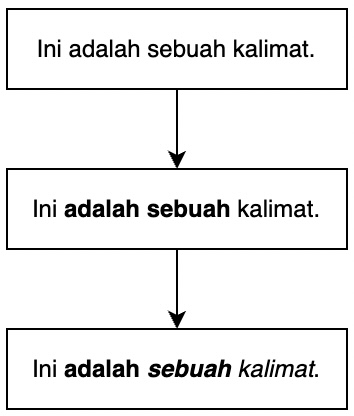
\includegraphics[scale=0.8]{assets/skripsi/richtext}
    \caption{Diagram Contoh Perubahan pada \textit{Rich Text Editor}}
    \label{fig:2:richtext}
\end{figure}

Pada editor kode atau teks yang bersifat kolaboratif setiap pengguna memiliki replikat dari suatu dokumen teks yang akan berakhir sama~\citep{Sun1998, Sun2004}. Setiap pengguna bebas melakukan penyuntingan secara bersamaan tanpa ada larangan tertentu. Operasi lokal kemudian akan diterapkan langsung pada replikat lokalnya tanpa ada jeda~\citep{attiya2016specification, Lv2015}. Operasi yang dilakukan oleh seorang pengguna akan dipropagasi pada setiap pengguna lain secara langsung dengan latensi minimal, sehingga sifat kolaborasi waktu nyata dapat terwujud. Terdapat beberapa algoritma yang akan mewujudkan konsistensi \textit{state} atau keadaan dokumen pada setiap replikatnya. Setiap operasi yang dilakukan oleh setiap pengguna akan menghasilkan dokumen identik yang merupakan hasil penyatuan atau konvergensi yang memenuhi suntingan operasi-operasi tersebut~\citep{Sun1998, Sun2004, Sun2019First, Sun2019third}. Operasi yang dilakukan bersifat komutatif, yang berarti terlepas dari urutan diterapkannya operasi pada suatu dokumen, hasilnya akan tetap sama melalui algoritma yang mewujudkan konsistensi ini~\citep{Sun1998}.

\section{OT (\textit{Operational Transformation})}
\label{subsec:OT}

Salah satu tantangan dalam menciptakan suatu sistem terdistribusi adalah untuk memiliki suatu basis atau struktur data yang nilainya konsisten untuk setiap klien dalam sistem tersebut. Salah satu struktur data yang menjadi fokus penelitian adalah dokumen \textit{plain text}. Metode OT (\textit{Operational Transformation}) dikembangkan dengan motivasi bagi setiap pengguna dalam suatu sistem terdistribusi dapat memiliki dokumen yang sama untuk setiap perubahan yang terjadi~\citep{Sun1998}. Dalam algoritma dasar OT, operasi yang digunakan adalah \texttt{insert(pos, c)}. Operasi tersebut memasukkan sebuah karakter $c$ pada indeks $\texttt{pos}$ dan setiap karakter yang posisi awalnya berada $\geq \texttt{pos}$ akan digeser ke indeks selanjutnya. Ada pula operasi \texttt{delete(pos)} atau menghapus sebuah karakter pada indeks \texttt{pos}~\citep{OTOverview1}. Unit operasi seperti \texttt{insert} dan \texttt{delete} ini merupakan unit dasar dari OT~\citep{OTOverview1}.

OT dibuat untuk menyelesaikan konflik operasi yang dapat terjadi tanpa mengetahui urutan terjadi antar setiap kliennya. OT secara garis besar bekerja melalui sebuah fungsi $T$, yang mentransformasikan dan menyesuaikan parameter suatu operasi $\op$ yang akan dilakukan pada suatu dokumen, berdasarkan operasi-operasi sebelumnya yang telah diterapkan pada dokumen tersebut. Terdapat dua sifat yang umumnya harus dipenuhi oleh suatu algoritma OT untuk bekerja, antara lain sebagai berikut~\citep{crdtLecture, OTOverview1, Li2004, Ressel1996}.

\begin{itemize}
    \item CP1/TP1 (\textit{Convergent Property} 1 atau \textit{Transformation Property} 1), yaitu $\op_1 \circ T(\op_2, \op_1) \equiv \op_2 \circ T(\op_1, \op_2)$.
    \item CP2/TP2 (\textit{Convergent Property} 2 atau \textit{Transformation Property} 2), yaitu $T(\op_{3},\op_{1}\circ T(\op_{2},\op_{1}))=T(\op_{3},\op_{2}\circ T(\op_{1},\op_{2}))$.
\end{itemize}


\begin{figure}[h]
    \centering
    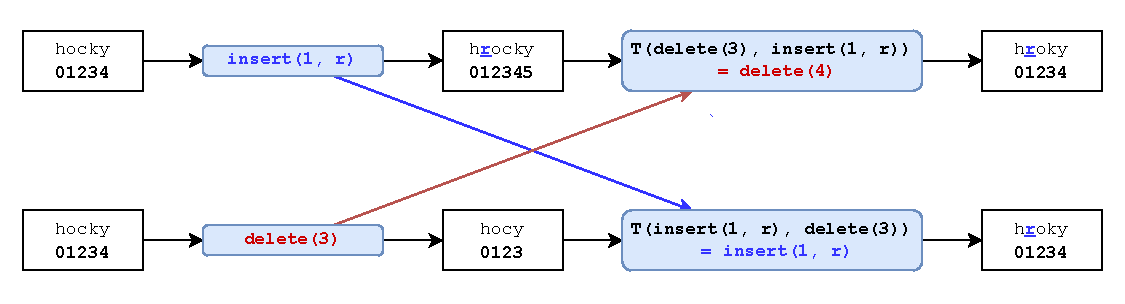
\includegraphics[scale=0.8]{assets/skripsi/OT}
    \caption{Diagram Ilustrasi TP1}
    \label{fig:OTschema}
\end{figure}

TP1 berarti bahwa dokumen yang diterapkan $\op_1$, dan dilanjutkan dengan penerapan operasi tranformasi $\op_2$ terhadap $\op_1$ haruslah ekuivalen dengan dokumen yang diterapkan $\op_2$ dan dilanjutkan dengan penerapan operasi transformasi $\op_1$ terhadap $\op_2$. TP1 diperlukan hanya jika dua operasi yang hendak diterapkan pada suatu replika diterapkan pada urutan yang berbeda. Implementasi algoritma \textit{operational transformation} yang memenuhi properti pertama ini cukup untuk membuat sebuah sistem terdistribusi dengan suatu sumber kebenaran yang berbasis \textit{client-server}. Pada suatu sistem \textit{operational transformation} yang tidak menggunakan TP2, salah satu syarat untuk mencapai konvergensi adalah setiap operasi hanya ditransformasikan pada satu sumber konteks yang sama~\citep{Xu2016}. Misalnya riwayat setiap operasi-operasi yang terdapat pada server dianggap sumber operasi yang mutlak untuk setiap klien~\citep{Vidot2000}. Saat klien menerima pembaharuan operasi, semua operasi lokal pada klien yang belum ditambahkan pada server akan ditransformasikan berdasarkan milik server. Operasi dari klien baru bisa di-\textit{append} ke server jika semua operasi yang terdapat pada server sudah dimiliki klien.

Properti lainnya yang harus dimiliki oleh \textit{operational transformation} ialah TP2 yang mengimplikasikan bahwa untuk tiga operasi berbeda, suatu operasi $\op_3$ yang ditransformasikan terhadap dua operasi yang sudah diterapkan lainnya, yaitu $\op_1$ dan $\op_2$ dengan sembarang urutan akan menghasilkan hasil transformasi yang sama. TP2 hanya dibutuhkan untuk sistem yang yang mengizinkan kedua operasi dijalankan pada dua \textit{state} dokumen yang berbeda. Berbeda halnya dengan TP1, \textit{update} secara \textit{concurrent} dapat terjadi untuk klien yang berbeda. Karena kerumitan algoritmanya dan beberapa penelitian dibuktikan salah dalam mengimplementasikan OT yang memenuhi TP2~\citep{OTOverview1}, CRDT dikenalkan sebagai alternatif dari OT sebagai metode untuk menjaga konsistensi dan kebenaran dari suatu dokumen atau data dalam sebuah jaringan sistem terdistribusi.

\section{CRDT (\textit{Conflict-Free Replicated Data Type})}

Sekitar awal tahun 2006, algoritma WOOT (\textit{WithOut Operational Transformation}) yang diteliti oleh~\cite{oster2005real} dikenalkan sebagai sebuah algoritma non-OT pertama untuk memastikan sifat konvergen dari replika teks pada editor kolaboratif sebagai alternatif dari OT. Tidak hanya itu, konsistensi dari \textit{intention} atau maksud dari sebuah operasi juga dapat dijaga~\citep{Li2004}. Misalnya ketika sebuah klien memasukkan sebuah karakter \texttt{X} di antara dua buah karakter \texttt{A} dan \texttt{B} pada sebuah \textit{string} dengan penomoran indeks dari $0$, ``\texttt{ABCDE}''. Operasi yang menjaga \textit{intention}, memiliki makna bahwa masukkan karakter \texttt{X}, sehingga \texttt{A} mendahului \texttt{X} dan \texttt{X} mendahului \texttt{B}. Dengan kata lain, operasi \texttt{insert} yang direpresentasikan sebagai operasi $\texttt{insert}(1, \texttt{X})$ pada OT, direpresentasikan sebagai operasi $\texttt{insert}(\texttt{A} \prec \texttt{X} \prec \texttt{B})$ pada algoritma ini. Dengan \texttt{A} dan \texttt{B} merupakan suatu objek yang memiliki ID pengenal yang bersifat unik untuk setiap karakter yang ada di dalam \textit{string}. Algoritma ini menjadi awal dari perkembangan struktur data CRDT yang secara formal didefinisikan untuk tidak hanya pada \textit{string}, namun berbagai struktur data abstrak lain pada tahun 2011 oleh~\cite{Shapiro2011}.

CRDT sendiri merupakan suatu tipe data abstrak untuk memelihara kecocokan dokumen pada beberapa replikanya dalam sebuah jaringan. Tipe data abstrak berarti semantiknya didefinisikan dari kumpulan nilai properti dan operasi fungsi atau prosedur. Oleh karena itu, implementasi dari CRDT untuk setiap operasinya bisa berbeda-beda, tapi menghasilkan \textit{behavior} yang sama untuk operasi yang sudah didefinisikan. CRDT didesain untuk disimpan pada setiap node atau \textit{peer} dalam sebuah jaringan. Oleh karena itu, implementasi CRDT yang efisien terhadap memori dan waktu juga menjadi pertimbangan dalam menggunakan struktur data ini. Struktur data ini memiliki karakteristik pada setiap replikanya yang bisa dimodifikasi tanpa berkoordinasi dengan replika lain, bila setiap replika dilakukan operasi yang sama tanpa memerhatikan urutannya, maka semuanya akan menghasilkan \textit{state} atau keadaan akhir yang sama~\citep{Shapiro2011, CRDToverview2}.

Salah satu dari contoh CRDT yang sederhana ialah \textit{unordered set} atau himpunan tak berurut~\citep{Shapiro2011}. Pada tipe data tersebut, setiap \textit{peer} dapat melakukan operasi \texttt{insert(v)}, yaitu menambahkan suatu elemen \texttt{v} ke dalam \textit{set} atau himpunan. Selanjutnya, ada pula operasi \texttt{erase(v)} yang akan menghapus elemen \texttt{v} dalam himpunan bila ada. Dalam penelitian ini, tipe data CRDT digunakan dalam proses pengolahan teks, sehingga operasi-operasi yang terkait dengan CRDT yakni serupa dengan yang disampaikan dengan operasi pada bagian~\ref{subsec:OT}, yakni \texttt{insert(pos, c)} serta \texttt{delete(pos)}.

Pada CRDT untuk teks biasa, setiap karakter akan memiliki ID berbeda. Saat melakukan operasi \texttt{insert}, data perubahan akan disertai dengan dua ID referensi karakter sebelum dan sesudahnya serta sebuah \textit{logical clock} untuk menandai urutan pemasukan karakter, seperti ide serupa yang disampaikan pada bagian awal subbab ini~\citep{oster2005real}. Terdapat beberapa cara yang umum diterapkan untuk merepresentasikan CRDT dan menangani kasus \textit{operasi} \texttt{delete}. Cara pertama ialah dengan menyimpan karakter yang sudah dihapus pada suatu dokumen selamanya, dan hanya akan ditandai sebagai ``terhapus'' teknik ini dikenal dengan istilah \textit{tombstone}~\citep{molli2006tombstone}. Pendekatan yang lainnya ialah dengan memberikan ID yang sudah terurut sesuai dengan urutan posisinya. Saat melakukan operasi \texttt{insert} pada suatu posisi tertentu, ID-nya akan lebih besar daripada ID karakter sebelumnya dan lebih kecil daripada ID sesudahnya. ID ini hendaknya bersifat dinamis dan ukurannya dapat bertambah seiring dengan bertambahnya karakter. Setiap ID disertai dengan pengenal tambahan berbeda untuk setiap kliennya yang memastikan ID-nya tidak ada yang duplikat. Saat melakukan operasi \texttt{delete}, node yang hendak dihapus tidak perlu disimpan pada suatu dokumen selamanya karena properti dari urutan ID ini.

Bila dibandingkan dengan OT yang hanya memanfaatkan fungsi transformasi operasi dan dokumennya direpresentasikan secara minimal sebagai \textit{array} karakter saja, CRDT membutuhkan struktur data tambahan untuk setiap karakter pada dokumen. Karakter tersebut akan diberikan ID dan dikenalkan sebagai objek. Karakter tersebut juga akan memiliki urutan penghubung (implisit maupun eksplisit) seperti yang disampaikan pada dua pendekatan CRDT di atas yang menyatakan urutan karakter sebelum dan sesudahnya. Terdapat pula perbedaan-perbedaan lainnya yang dijelaskan lebih lanjut pada subbab~\ref{sec:perbandingan} selanjutnya.

\section{Perbandingan Lanjut CRDT dan OT}
\label{sec:perbandingan}

Industri teks editor kolaboratif waktu nyata masih didominasi oleh \textit{operational transformation} meskipun CRDT memiliki kompleksitas dan efisiensi yang diklaim lebih optimal dibandingkan OT~\citep{Sun2019third}. Tidak ada definisi perbedaan yang terlalu jelas untuk kapan suatu algoritma menggunakan OT dan CRDT, karena pada dasarnya keduanya merupakan transformasi untuk mencapai komutativitas dari fungsi yang direalisasikan menggunakan parameter yang berbeda. Pada CRDT, operasi diubah menjadi representasi ID atau tanda pengenal lain, kemudian dikembalikan ke bentuk posisinya lagi setelah diaplikasikan, sementara pada OT, operasi dinyatakan dengan posisi dari karakternya langsung.

Pendekatan \textit{operational transformation} berlangsung dan terfokus pada algoritma transformasi fungsi yang mengelola dan mengendalikan operasi dari setiap kliennya yang berlangsung bersamaan. Sementara CRDT terfokus pada konten seperti urutan objek, operasi yang berbasis \textit{identifier} atau ID pengenal, dan skema atau representasi lain dalam menyatakan operasi penyuntingan~\citep{Sun2019Second, Sun2019First}. Hal ini membuat struktur data CRDT lebih spesifik penggunaannya untuk tipe data abstrak tertentu, misalnya untuk \textit{set}, \textit{map}, dan teks memiliki implementasi dan algoritmanya masing-masing. Perbedaan pendekatan ini menyebabkan kompleksitas dari kedua metode ini berbeda. Pada OT, variabel kompleksitas dipengaruhi oleh banyaknya operasi yang berlangsung secara bersamaan, dan tidak ada biaya untuk merepresentasikan dan memanipulasi karakter pada teks ke dalam bentuk objek dan struktur datanya. Pada CRDT, variabel kompleksitas ini akan semakin besar dan berbanding lurus dengan ukuran dokumen atau banyaknya konten. Selain itu, biaya \textit{overhead} kompleksitas waktu dan memori inisialisasi untuk \textit{peer} baru yang masuk ke dalam jaringan juga cenderung lebih besar dibandingkan OT.

Bila dilihat dari pembuktian dari kebenaran algoritmanya, CRDT memiliki kerumitan yang lebih tinggi dibandingkan OT karena adanya perlakuan khusus terhadap \textit{state} kontennya~\citep{Sun2019Second}. Terdapat banyak sekali variasi algoritma dari CRDT, sehingga pembuktian sifat konvergennya cenderung lebih sulit dibandingkan OT yang kriteria kebenarannya properti-properti khusus yang sudah dibuktikan pada penelitian-penelitian sebelumnya~\citep{OTOverview1, Sun2004, oster2005real}. Berdasarkan penelitian~\cite{Sun2019Second}, kompleksitas waktu yang diperlukan untuk sistem OT yang merupakan {state-of-the-art} saat ini dalam mengaplikasikan operasi \textit{remote} adalah $O(c)$ dan operasi lokal ialah $O(1)$, dan kompleksitas memori $O(c)$ atau $O(c \cdot m)$ dengan $c$ adalah banyaknya banyaknya operasi bersamaan yang akan ditransformasikan (dalam praktisnya nilainya sangat kecil $(c \leq 10)$ karena operasi berlangsung dalam waktu nyata) dan $m$ adalah banyaknya pengguna dalam jaringan (umumnya $m \leq 5$). Sementara pada CRDT, definisikan $C$ sebagai ukuran konten (tanpa \textit{tombstone}) dan $C_t$ sebagai konten seumur dokumen (dengan \textit{tombstone}). Kompleksitas waktu untuk setiap operasinya dapat berkisar antara $O(C_{t}^{2})$, $O(C_{t})$, hingga $O(1)$ untuk CRDT berbasis \textit{tombstone}, dan $O(\log C)$ untuk solusi yang tidak berbasis \textit{tombstone}. Sementara kompleksitas optimal memorinya bisa mencapai $O(C)$ untuk solusi berbasis \textit{non-tombstone} dan \textit{tombstone} dengan \textit{garbage-collection}. Nilai dari $C$ umumnya berkisar antara $10^3 \leq C \leq 10^6$ untuk dokumen biasa pada umumnya. Implementasi dari CRDT dan variasinya dibahas lebih lanjut pada subbab~\ref{sec:penelitian_terkait}.

\section{Penelitian Terkait}
\label{sec:penelitian_terkait}

Penelitian ini menggunakan \textit{library} Yjs yang mengimplementasikan algoritma YATA (\textit{Yet Another Transformation Approach}) untuk CRDT-nya. YATA menggunakan \textit{linked-list} dalam merepresentasikan datanya dan menggunakan sistem \textit{tombstone} dengan proses \textit{garbage-collector} dalam mengoptimisasi objek konten yang dinyatakan terhapus. Dalam algoritma YATA yang diteliti oleh~\cite{Nicolaescu2016yjs}, operasi \texttt{insert} dinyatakan sebagai menambahkan sebuah objek $o(id, left, right, isDeleted, content)$ ke \textit{linked-list}. Tanda pengenal $id$ berisikan pasangan berurut ID \textit{peer} dan \textit{logical timestamp} berupa operasi ke berapa yang telah dilakukan \textit{peer} tersebut. Properti $left$ dan $right$ masing-masing merupakan variabel yang menandakan $id$ untuk objek yang berada di sebelah kiri dan kanannya saat operasi \texttt{insert}. Bagi teks editor untuk mengetahui keberadaan objek tersebut, terdapat properti $isDeleted$ yang merupakan nilai \textit{boolean} yang menunjukkan sudah terhapus atau tidaknya objek tersebut, serta properti $content$ yang merupakan \textit{string} yang berisi konten data dari objek tersebut.

Optimisasi pada Yjs terdapat pada properti $content$ yang dapat berupa \textit{string} atau kumpulan karakter. Saat ada operasi \texttt{insert} di antara dua konten dalam objek yang sama, objek tersebut akan dibagi menjadi dua objek lain. Sehingga dalam representasinya, \textit{logical timestamp} juga akan menyimpan informasi panjang konten di objek saat ini. Operasi penghapusan dilakukan dengan secara sederhana menandai objek tersebut menjadi terhapus. Untuk detail implementasi dan kompresi lebih lanjut disampaikan pada penelitian YATA~\citep{Nicolaescu2016yjs}.

Yjs merupakan \textit{library} yang baru populer digunakan pada tiga tahun terakhir selama penelitian ini. Terdapat beberapa implementasi algoritma lain seperti Logoot yang menggunakan \textit{vector clock} pada \textit{timestamp} objeknya. \textit{Vector clock} atau \textit{state vector} secara sederhana merupakan sebuah vektor yang merepresentasikan versi dari setiap \textit{peer} dalam jaringan. Dalam Logoot, operasi penghapusan dilakukan langsung dengan menghapus objek tanpa perlu menyimpan \textit{tombstone}~\citep{weiss2009logoot}.

CRDT YATA melanjutkan ide awal dari CRDT LSeq (Linear Sequences) yang ID pengenalnya tidak menggunakan \textit{timestamp}. Permasalahan dari algoritma ini ialah dapat terjadinya \textit{interleaving}, yakni urutan untuk operasi \texttt{insert} yang dilakukan bersamaan tidak memiliki komparator lanjutan (hanya \textit{partial order}) saat adanya konkurensi yang terjadi ketika terdapat lebih dari satu karakter memiliki penunjuk objek \textit{left} dan \textit{right} sama pada dua \textit{peer} berbeda~\citep{kleppmann2019interleaving, nedelec2013lseq}. YATA menyelesaikan masalah ini dengan menambahkan \textit{logical timestamp} untuk setiap kliennya.

Alternatif dari YATA, yaitu RGA (Replicated Growable Array) menyelesaikan masalah \textit{interleaving} pada LSeq dengan menggunakan pasangan berurut ID \textit{peer} dan \textit{timestamp global} yang didapat dari \textit{timestamp} selanjutnya dari \textit{timestamp} operasi terkecil pada CRDT. Dalam praktisnya, algoritma ini memiliki berbagai optimisasi lebih terlepas dari algoritma yang disampaikan pada penelitian formalnya. Misalnya penambahan \textit{garbage collector}, kompresi data antar jaringan, dan penyimpanan objek dalam memori yang memengaruhi performanya.
\clearchapter
%-----------------------------------------------------------------------------%
\chapter{\babTiga}
\label{bab:3}

Bab ini secara umum memaparkan tentang metodologi penelitian yang ditempuh dalam mengembangkan sistem PeerToCP yang mencakup pendekatan, rincian tahapan, serta aspek-aspek yang akan diujikan pada sistem. Pendekatan dan tahapan penelitian penting untuk memberikan penjelasan terhadap langkah-langkah saintifik yang ditempuh dalam penelitian ini. Penjelasannya lebih lanjut dijelaskan pada subbab~\ref{sec:pendekatan} berikut.

\section{Pendekatan dan Tahapan Penelitian}
\label{sec:pendekatan}
Penelitian ini dilaksanakan dengan pendekatan \textit{experimental research}. Data kuantitatif dan kualitatif akan diukur untuk setiap variasi dari aplikasi PeerToCP yang memiliki implementasi \textit{business logic} di atas UI (\textit{user interface}) atau antarmuka pengguna yang sama. Variabel bebas dari penelitian ini difokuskan pada basis arsitektur dari jaringan PeerToCP serta metode resolusi dan sinkronisasi data yang digunakan. Variabel terikat yang akan diukur dari penelitian ini disusun berdasarkan aspek-aspek sistem. Data kuantitatif akan didapat dari hasil \textit{benchmarking} dan akan dianalisis. Data kualitatif akan didapatkan melalui paparan deskriptif secara objektif terhadap sistem. Bagan berikut memberikan gambaran besar tahapan penelitian yang dilaksanakan.

\begin{figure}
    \centering
    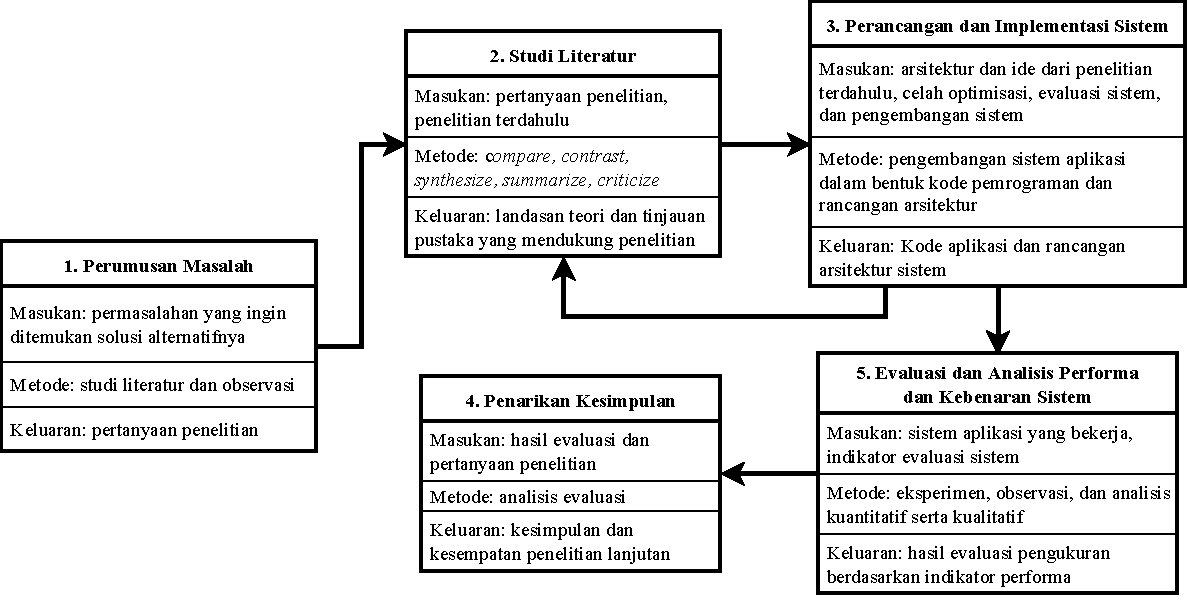
\includegraphics[scale=0.7]{assets/skripsi/Metode_Penelitian}
    \caption{Bagan Alur Penelitian}
    \label{bagan}
\end{figure}

Perumusan masalah dalam penelitian ini dilatarbelakangi oleh potensi penggunaan teknologi web berupa WebRTC dan beberapa variasi algoritma sinkronisasi data dalam suatu jaringan terdistribusi yang memiliki keuntungan dan kerugiannya masing-masing. Ide ini dikembangkan pula melalui kebutuhan sistem yang mempermudah melakukan kegiatan pemrograman kompetitif, yaitu suatu IDE (\textit{Integrated Development Environment}) sederhana yang memungkinkan adanya pengembangan kode secara kolaboratif dalam waktu nyata dan penjalanan program yang dapat dilakukan pada suatu klien di dalam jaringan yang dapat diakses oleh setiap klien lain di dalam jaringan pula. Dari rumusan masalah tersebut, akan didapatkan pertanyaan-pertanyaan yang mendasari penelitian ini.

Melalui masukan pertanyaan, dilakukan studi literatur terhadap teknologi-teknologi dan penelitian terdahulu. Tahap ini menghasilkan landasan teori dan tinjauan pustaka sebagai dasar pengetahuan. Studi literatur dilakukan dengan membandingkan penelitian terkait yang serupa, dari segi performa, kerumitan implementasi, cara kerja, dan bukti kebenaran teknologi atau algoritma tertentu. Studi literatur ini berguna untuk mengetahui seberapa jauh kemajuan teknologi yang diteliti pada topik ini. Selanjutnya, penelitian dilanjutkan dengan perancangan dan implementasi sistem aplikasi PeerToCP. Terdapat tiga variasi dari sistem aplikasi PeerToCP yang akan diujikan, yaitu variasi dengan metode OT (\textit{operational transformation}) berbasis \textit{client-server}, CRDT (\textit{conflict-free replicated data types}) berbasis \textit{client-server}, dan CRDT berbasis \textit{peer-to-peer}. Detail implementasi dan arsitektur aplikasi akan dijelaskan secara detail pada Bab~\ref{bab:4} Implementasi. Sistem yang telah dikembangkan kemudian akan dilakukan evaluasi secara objektif berdasarkan aspek-aspek tertentu yang menrepresentasikan performa dan skalabilitas aplikasi. Poin-poin aspek yang disampaikan pada subbab~\ref{sec:evaluasi} selanjutnya disampakan untuk memberikan konteks perbandingan yang jelas antara suatu implementasi dengan yang lainnya.

\section{Metode dan Skenario Evaluasi}
\label{sec:evaluasi}

Dari observasi terhadap beberapa aplikasi \textit{real-time collaborative} lain, evaluasi pada penelitian ini menturutsertakan beberapa aspek esensial untuk setiap variasi dari aplikasi PeerToCP, antara lain ialah sebagai berikut.

\begin{enumerate}
    \item \textit{Correctness}, mengindikasikan kebenaran untuk setiap variasi implementasi PeerToCP. Aspek ini dipilih untuk menentukan bahwa setiap replika data yang dijaga kesamaannya berakhir konvergen dan identik.
    \item \textit{Lightweight}, aplikasi berjalan dengan sumber daya atau \textit{resource} minimal dan tidak mengganggu jalannya aplikasi lain pada suatu sistem operasi. Suatu aplikasi hendaknya tidak menggunakan \textit{resource} yang berlebihan dalam mencapai tujuannya, hal ini dapat berdampak langsung terhadap minat penggunaan aplikasi ke depannya.
    \item \textit{Responsiveness}, sinkronisasi replika data pada setiap klien dilakukan dalam latensi yang rendah dan layak guna. Setiap klien yang menggunakan suatu aplikasi \textit{real-time collaborative} seharusnya mendapatkan jeda minimal untuk memberikan pengalaman pengguna atau \textit{user experience} waktu nyata.
    \item \textit{Local-First}, operasi diterapkan pada replika lokal secara langsung setelah diberikan pengguna tanpa perlu berhubungan dengan klien atau server lain di dalam jaringan.
    \item \textit{Scalability}, aspek ini berhubungan langsung dengan setiap aspek lain, karena penggunaan arsitektur \textit{peer-to-peer} pada awalnya memiliki motivasi untuk meningkatkan ketersediaan layanan dengan mengurangi beban pada server. Performa dari aplikasi berpengaruh terhadap banyaknya klien atau pengguna dalam suatu jaringan, sehingga aspek ini penting untuk diperhatikan dalam sistem terdistribusi aplikasi~\citep{leibnitz2007peer}.
\end{enumerate}

Data kuantitatif dan kualitatif yang diperoleh pada proses \textit{benchmarking} ini akan dianalisis. Setelahnya, hasil analisis akan disimpulkan dengan memberikan kesempatan optimisasi dan pengembangan untuk penelitian-penelitian selanjutnya.

\clearchapter
%-----------------------------------------------------------------------------%
\chapter{\babEmpat}
\label{bab:4}

Bab ini menjelaskan detail arsitektur dan implementasi dari aplikasi PeerToCP. Selain itu, terdapat penjelasan singkat serta alasan pemilihan beberapa teknologi, termasuk \textit{library} dan \textit{modul} yang digunakan dalam implementasi, diikuti dengan \textit{usecase} atau fitur sistem. Bab ini juga memaparkan detail skenario pengujian dan metode evaluasi disusun berdasarkan aspek-aspek sistem pada variasi yang akan dibandingkan.

\section{\textit{Library} dan \textit{Framework} Terkait}

Terdapat beberapa modul dan \textit{library} pihak ketiga yang dimanfaatkan dalam pengembangan sistem aplikasi PeerToCP yang dibahas dalam penelitian ini. Berbagai \textit{framework} dan \textit{library} ini merupakan hasil penelitian dan implementasi oleh para pengembang sebelumnya. Pemilihan penggunaan setiap teknologi ini dipertimbangkan dengan alasan tertentu, salah satunya adalah Electron, yang menjadi basis pengembangan aplikasi \textit{desktop} pada PeerToCP.

\subsection{\textit{Framework} Utama dan Komponen Editor Kode}

Electron merupakan salah satu \textit{framework} \textit{desktop} yang sistem kerja pengembangannya serupa dengan komponen web. Bagian tampilan atau \textit{frontend} dari Electron memanfaatkan aplikasi \textit{Chromium} yang dapat mengolah bahasa \textit{markup} web, seperti HTML (\textit{HyperText Markup Language}), CSS (\textit{Cascading Style Sheets}), serta JavaScript. Bagian belakang atau \textit{backend} dari Electron berjalan dengan \textit{environment runtime} Node.js~\citep{kredpattanakul2018transforming, miglanielectron}. Node.js merupakan bahasa yang menggunakan \textit{syntax} yang serupa dengan JavaScript dan dapat dikompilasi melalui kompilator yang disebut V8 engine~\citep{tilkov2010node}.

Salah satu keuntungan menggunakan Electron adalah aplikasinya yang bersifat \textit{cross-platform} atau dapat berjalan di beragam sistem operasi, seperti Windows, GNU/Linux, atau MacOS. Electron mengizinkan akses berbagai macam fungsi antarmuka sistem operasi, seperti memanggil subproses pada sistem dan menulis berkas. Karena \textit{frontend}-nya yang menggunakan bahasa web pula, aplikasi yang dibuat dengan Electron cenderung lebih mudah untuk dipindahkan dan diadaptasi dengan fungsi terbatas pada web. Selain Electron, masih terdapat beberapa alternatif \textit{desktop-based framework} lain seperti Qt yang berbasis C++ dan Tauri yang berbasis Rust. Pemilihan Electron dipilih karena beberapa \textit{library} \textit{operational transformation}, CRDT, WebSocket, dan WebRTC yang umum digunakan sudah tersedia implementasinya dalam JavaScript dan dapat digunakan melalui Node.js.

Aplikasi dengan \textit{framework} Electron memiliki proses utama atau dikenal dengan istilah \textit{main process} yang akan berjalan saat aplikasi dimulai~\citep{electron}. Setiap jendela tampilan yang dibuka akan diwakili oleh sebuah proses pengolah atau \textit{renderer process}. Tampilan PeerToCP direpresentasikan oleh sebuah jendela editor kode dengan \textit{renderer process}-nya yang memiliki mekanisme untuk sewaktu-waktu berkomunikasi dengan \textit{main process} dan membuat jendela \textit{shell} yang mengandung program berjalan hasil kompilasi. \textit{Renderer process} bertanggung jawab untuk mengolah konten \textit{frontend} yang serupa dengan komponen-komponen web. Dalam penelitian ini, salah satu komponen utama yang ditampilkan pada jendela utama PeerToCP ialah CodeMirror.

CodeMirror digunakan dalam komponen editor kode dan berperan sebagai media interaksi pengguna dengan sistem aplikasi pada \textit{frontend}. CodeMirror sendiri disusun untuk dapat di-\textit{render} oleh peramban web dan mengolah teks dengan sistem \textit{state} disertai operasi perubahan yang bersifat modular. CodeMirror menyediakan banyak ekstensi, aksesibilitas tinggi, serta dukungan untuk berbagai macam bahasa pemrograman. CodeMirror dimanfaatkan pula sebagai perantara dengan Yjs, sebuah \textit{library} CRDT yang sudah diintegrasikan dengan CodeMirror.

\subsection{Komponen Kolaborasi}

Yjs merupakan sebuah \textit{library} yang mengimplementasi CRDT yang disebut YATA (\textit{Yet Another Transformation Approach})~\citep{Nicolaescu2016yjs}. Yjs terdiri dari beberapa bagian, yaitu YDocs yang merupakan bagian utama implementasi berbagai struktur data untuk CRDT, ada pula YText yang merupakan variasi CRDT untuk operasi-operasi pada teks, serta YMap dan YArray yang dikombinasikan untuk menyimpan \textit{shell} dan riwayatnya. Dalam penelitian ini, digunakan tiga struktur data CRDT tersebut yang abstraksinya berbeda-beda.

Yjs juga merupakan \textit{library} yang tidak terpaku pada sebuah arsitektur. Dalam penelitian ini digunakan dua \textit{provider} jaringan yang dapat berintegrasi dengan YDocs, yaitu YWebRTC dan YWebSocket. Kedua provider ini masing-masing mengintegrasikan YDocs dengan jaringan berarsitektur \textit{full-mesh peer-to-peer} serta \textit{client-server} secara berturut-turut. Yjs memiliki banyak pengembang aktif dan hingga kini masih di-\textit{maintain} dan dikembangkan, sehingga \textit{library} Yjs dipilih dalam penelitian ini.

Untuk variasi \textit{operational transformation} dari PeerToCP, penelitian ini memanfaatkan ekstensi \textit{collaborative editing} dari CodeMirror yaitu @codemirror/collab. \textit{Provider} jaringan untuk arsitektur \textit{client-server} yang dikembangkan untuk metode ini menggunakan \textit{library} rpc-websockets yang dimodifikasi sehingga dapat dimanfaatkan untuk melakukan \textit{broadcast}, \textit{specific-messaging} ke klien tertentu, serta fungsionalitas pemanggilan RPC (\textit{Remote-Procedure Call}) berbentuk \textit{promise} secara \textit{asynchronous} dan \textit{non-blocking}.

Pada variasi PeerToCP dengan metode OT, penyimpanan \textit{shell} diimplementasi menggunakan prinsip OT dan sifat \textit{append-only array} untuk menyederhanakan kompleksitas program. Operasi-operasi yang dapat dilakukan pada \textit{shell} ialah berupa \textit{keystroke} masukan pengguna. Secara khusus, beberapa \textit{keystroke} diperlakukan oleh terminal secara harfiah dan program yang berjalan pada \textit{shell} tersebut sendiri yang harus menangani bagaimana \textit{keystroke} tersebut akan diperlakukan. Misalnya, operasi penghapusan atau melakukan \textit{backspace} secara bawaan pada masukan \textit{shell} diartikan sebagai menambahkan tiga karakter ``$\texttt{\char`\\ b \char`\\ b}$'' (tanpa tanda petik) atau ekuivalen dengan memindahkan \textit{cursor} ke kiri, memasukkan karakter \textit{whitespace}, dan memindahkan \textit{cursor} ke kiri kembali. Dalam penelitian ini, aspek kolaborasi dari \textit{shell} memperlakukan setiap klien untuk memberikan \textit{keystroke} pada satu kanal yang sama tanpa \textit{positional cursor} ganda seperti pada editor kode.

\subsection{Komponen \textit{Shell}}

Untuk memenuhi komponen penjalanan program pada suatu \textit{shell} yang dapat diakses oleh setiap klien dalam jaringan, dibutuhkan suatu \textit{library} untuk mengakses sistem operasi untuk melakukan kompilasi terhadap kode. Kompilasi merupakan proses mengonversi kode dari bahasa dengan level yang lebih tinggi dan dapat dimengerti oleh manusia menjadi kode biner yang dapat dimengerti oleh mesin~\citep{aho1985compilers}. Pada penelitian ini, selain editor kode yang bersifat kolaboratif, proses kompilasi berkas kode tunggal juga dapat dilakukan oleh setiap pengguna. Proses kompilasi ini membutuhkan kompilator yang terpasang pada suatu sistem operasi. Pada Node.js, salah satu \textit{library} yang dapat digunakan untuk mengaksesnya ialah Node-pty.

Node-pty merupakan \textit{library} Node.js yang menyediakan antarmuka untuk melakukan \textit{fork} proses dengan deskriptor berkas \textit{pseudoterminal}. Node-pty mengizinkan adanya aliran data untuk baca dan tulis dengan proses berjalan pada kernel. Node-pty berguna untuk menjalankan berkas hasil kompilasi yang bersifat CLI (\textit{Command Line Interface}) yang tidak memiliki tampilan grafik untuk pengguna. Node-pty dipilih karena banyak digunakan dan bersifat \textit{cross-platform}. Aplikasi ini juga membutuhkan bagian \textit{frontend} untuk menampilkannya, dan digunakan Xterm.js. \textit{Library} ini merupakan salah satu komponen yang menampilkan terminal pada web. Xterm.js memiliki antarmuka yang bisa menerima dan meneruskan data dari peramban (\textit{browser}) yang dapat dihubungkan dengan sebuah proses berjalan pada sistem. Xterm.js dikembangkan tanpa memerlukan dependensi, sehingga dipilih dalam pengembangan sistem ini.

\section{Desain Sistem}

Aplikasi PeerToCP didesain sebagai sebuah aplikasi \textit{desktop-based}, yang berarti dijalankan secara langsung pada komputer. Pilihan ini dipertimbangkan untuk mempermudah akses secara luring, sehingga tidak dibutuhkan koneksi internet untuk mengakses aplikasi. Selain itu, fitur kompilasi pada suatu \textit{peer} memerlukan akses \textit{system-call} yang tidak disediakan pada API peramban web~\citep{v8, spidermonkey}. Peramban web ditetapkan seperti ini untuk mencegah \textit{script} yang berpotensi menyerang sistem operasi komputer tidak dapat dijalankan secara langsung. \textit{Diagram activity} yang menunjukkan garis besar alur penggunaan aplikasi dapat dilihat pada gambar~\ref{fig:activity}.

\begin{figure}
    \centering
    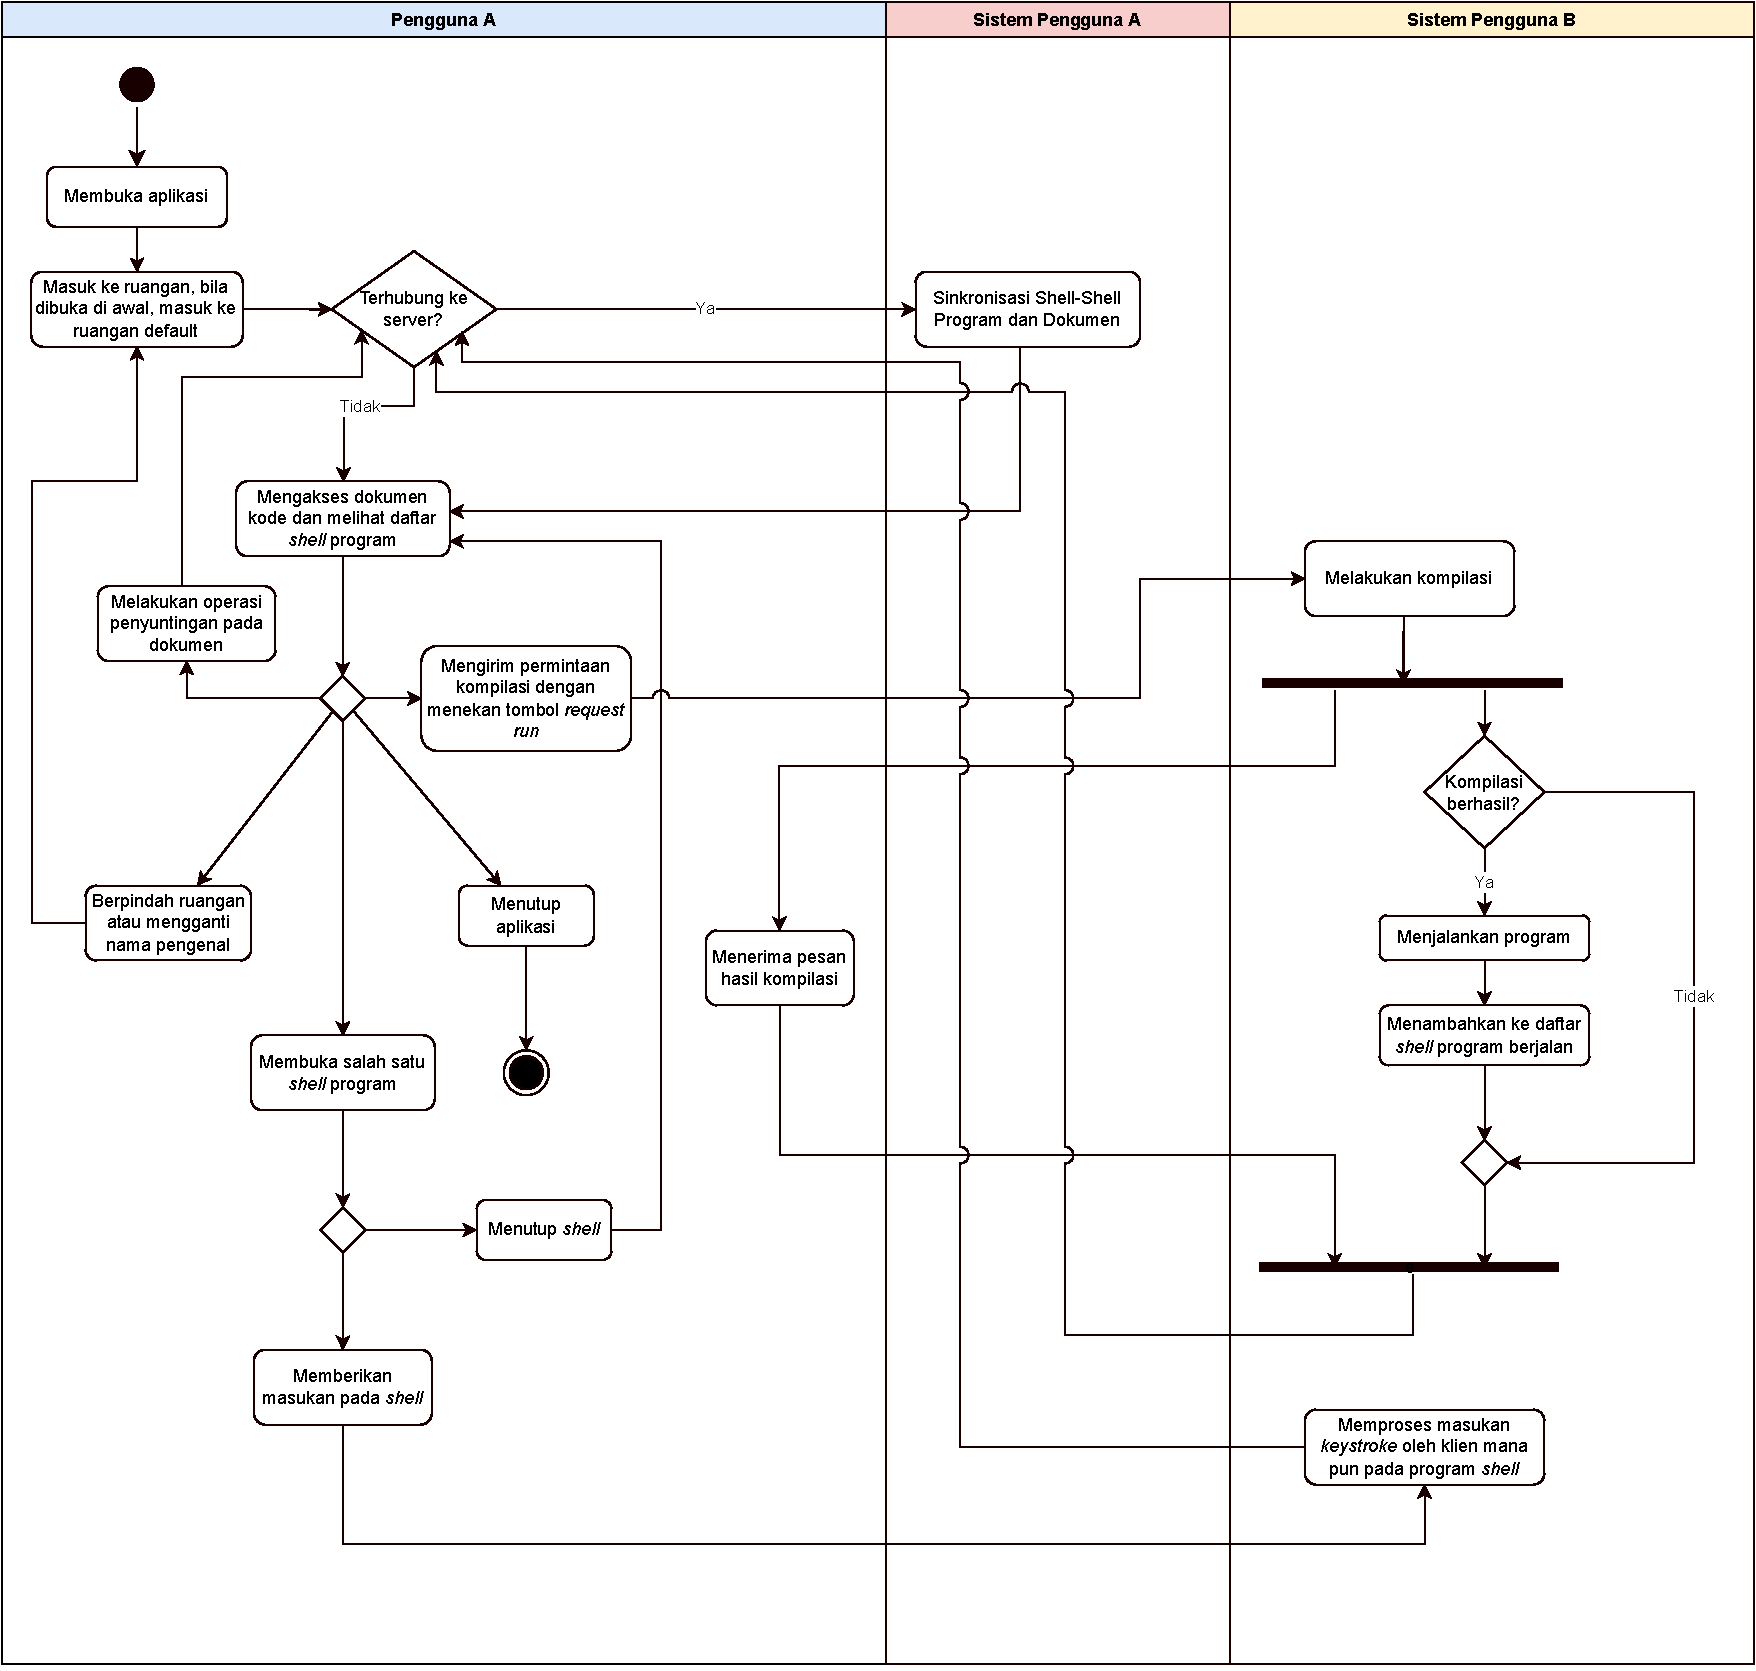
\includegraphics[scale=0.5]{assets/skripsi/Activity_Diagram}
    \caption{\textit{Activity Diagram} Alur Penggunaan Secara \textit{High Level}}
    \label{fig:activity}
\end{figure}

Saat pengguna membuka aplikasi, pengguna akan diarahkan untuk masuk ke ruangan awal secara \textit{default}. Pengguna dapat melakukan operasi-operasi penyuntingan pada dokumen dan sinkronisasi dilakukan secara terus-menerus dengan \textit{publish-subscribe design pattern} sehingga memberikan respons tanpa perlu mengecek atau \textit{polling} saat terjadi \textit{update} yang terjadi antarpengguna. \textit{Request} atau permintaan kompilasi dapat diajukan kepada pengguna mana pun pada sebuah jaringan, termasuk permintaan kepada pengguna tersebut sendiri. Aplikasi PeerToCP akan mencoba mengirimkan pesan kepada pengguna yang ditentukan tanpa intervesi dari pengguna lain dalam jaringan. Apabila permintaan berhasil diterima, sistem pada penerima permintaan akan melakukan proses kompilasi dan memasukkan \textit{shell} program berjalan dengan ID tertentu ke daftar \textit{shell} yang dapat diakses oleh setiap klien dalam jaringan. Daftar \textit{shell} dan kontennya ini disimpan dalam bentuk \textit{object} pada \textit{JavaScript}.

Pada gambar~\ref{fig:activity}, perilaku sinkronisasi \textit{shell}-\textit{shell} pada program dan dokumen dilakukan bergantung dengan variasi implementasi dari program. Pada arsitektur \textit{client-server}, sistem aplikasi pengguna A akan berhubungan dan melakukan sinkronisasi dengan server. Sementara pada arsitektur \textit{peer-to-peer}, sistem aplikasi pengguna A akan berhubungan langsung dan melakukan sinkronisasi dengan \textit{peer} lain. Selain itu, permintaan dan transmisi pesan hasil kompilasi dilakukan melalui pengiriman pesan secara langsung pada arsitektur \textit{peer-to-peer}, namun harus melalui perantara server pada arsitektur \textit{client-server}.

\section{CRDT (\textit{Conflict-Free Replicated Data Type}) Berbasis \textit{Peer-To-Peer} dan \textit{Client-Server}}
\label{sec:desain_crdt}

Implementasi CRDT pada dua skenario arsitektur dalam penelitian ini menggunakan \textit{library} CRDT Yjs. Setiap \textit{peer} atau klien memiliki replika yang direpresentasikan dalam tipe data YDocs. YDocs dapat terdiri dari beberapa CRDT \textit{nested} untuk menyimpan data-datanya, dalam penelitian ini \textit{shell} direpresentasikan sebagai sebuah CRDT YMap yang memetakan \textit{id} sebuah \textit{shell} ke sebuah CRDT YArray yang berisi kontennya. Implementasi dari variasi \textit{peer-to-peer} menggunakan \textit{library} penyedia jaringan YWebRTC yang telah dimodifikasi dengan antarmuka untuk mengirim pesan ke \textit{peer} tertentu melalui jaringan RTCDataChannel seperti yang ditunjukkan pada gambar ilustrasi~\ref{crdt-p2p}. \textit{Keystroke} yang diberikan oleh sebuah \textit{peer} tertentu akan dikirim langsung pada \textit{peer host} yang menjalankan programnya, kemudian \textit{peer host} akan menambahkan hasil \textit{keystroke} pada struktur \textit{array} yang berkorespondensi dengan \textit{shell} yang berisi program tersebut.

\begin{figure}
    \centering
    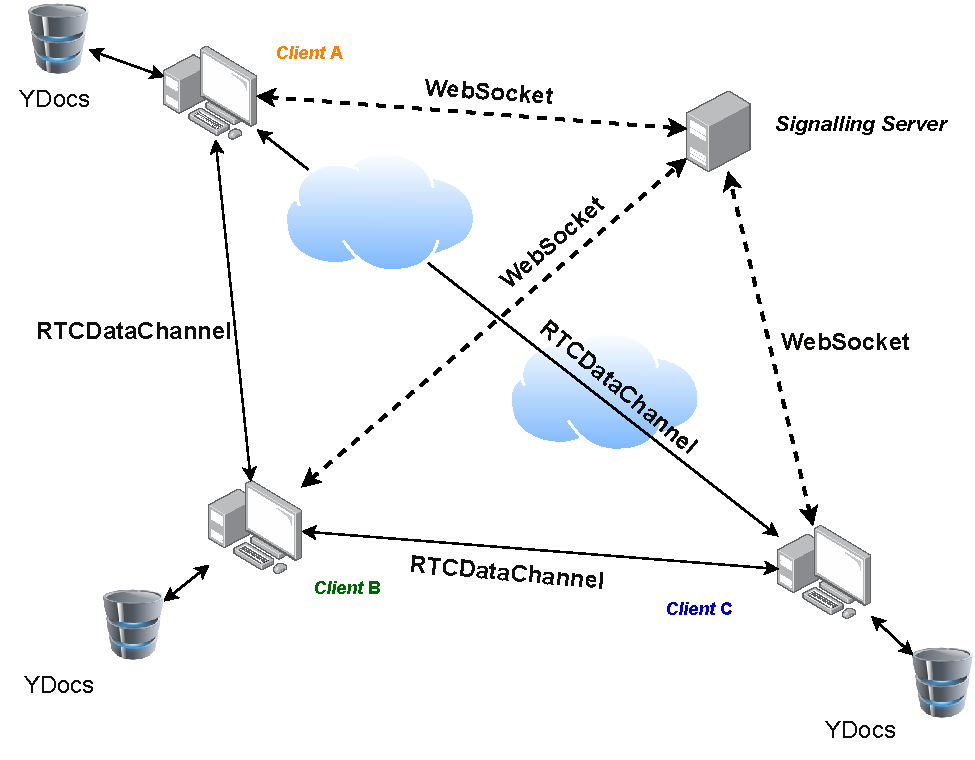
\includegraphics[scale=0.65]{assets/skripsi/Arsitektur_WebRTC_CRDT}
    \caption{Arsitektur \textit{Peer-To-Peer} yang Menggunakan WebRTC dengan WebSocket \textit{Signalling} Server dan CRDT}
    \label{crdt-p2p}
\end{figure}

\begin{figure}
    \centering
    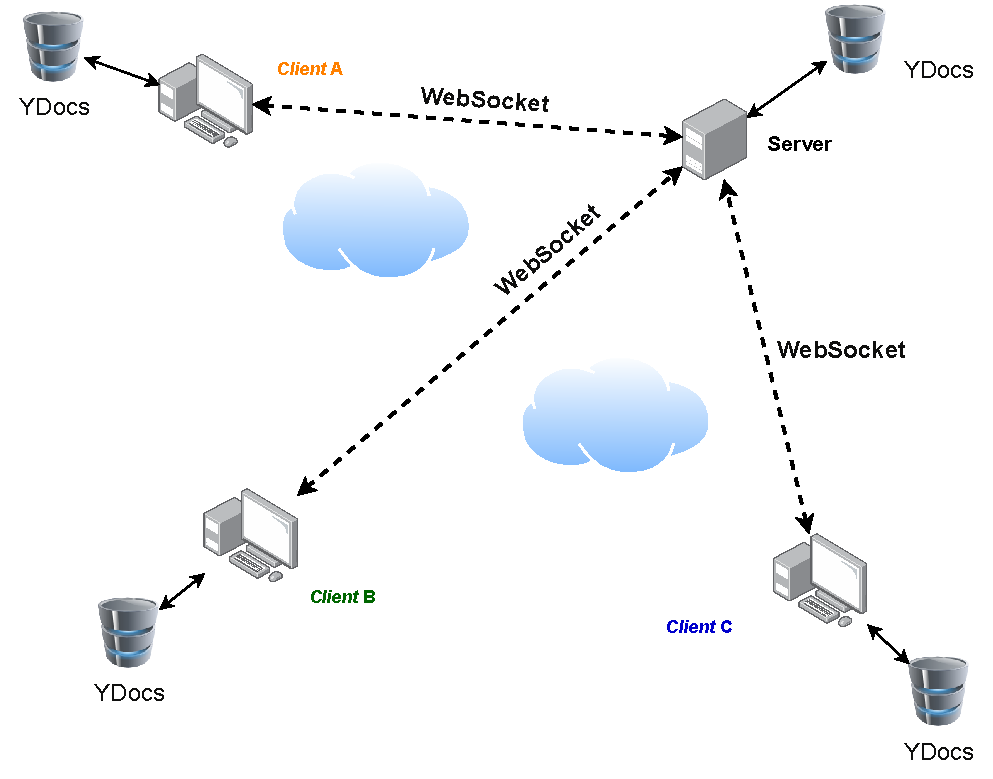
\includegraphics[scale=0.65]{assets/skripsi/Arsitektur_WebSocket_CRDT}
    \caption{Arsitektur \textit{Client-Server} yang Menggunakan WebSocket dan \textit{CRDT}}
    \label{crdt-cs}
\end{figure}

Perbedaan antara kedua implementasi arsitektur CRDT ini terdapat pada \textit{provider} atau penyedia jaringannya. Arsitektur \textit{client-server} diilustrasikan melalui gambar~\ref{crdt-cs}. Pada arsitektur \textit{client-server}, penelitian ini menggunakan \textit{library} YWebSocket yang telah dimodifikasi pula untuk dapat mengirim pesan kepada klien tertentu dalam sebuah jaringan melalui server. Penyedia jaringan memberikan abstraksi bagi setiap \textit{peer} atau klien dalam sebuah jaringan terdistribusi untuk berhubungan satu sama lain. Terdapat fitur tambahan bagi server pada arsitektur \textit{client-server} untuk dapat melakukan persistensi data. Persistensi ini mengizinkan untuk server menyimpan salah satu replika dari dokumen, sehingga dokumen masih akan tetap ada walaupun tidak ada klien yang terhubung. Selain CRDT, arsitektur \textit{client-server} digunakan bersama metode \textit{operational transformation} untuk menjaga kesamaan replika dalam suatu jaringan sistem terdistribusi. Variasi PeerToCP dengan \textit{operational transformation} yang hanya memenuhi \textit{transformation property} 1 berbasis \textit{client-server} menjadi salah satu variasi yang dibandingkan dalam penelitian ini.

\section{Metode \textit{Operational Transformation} Berbasis \textit{Client-Server}}
\label{sec:design_ot}

Untuk suatu dokumen yang hanya menyimpan teks biasa, operasi \textit{operational transformation} yang hanya memenuhi sifat TP 1 dapat diimplementasi dengan sederhana dalam arsitektur \textit{client-server}. Aplikasi PeerToCP dengan variasi ini menggunakan \textit{library} @codemirror/colab yang mengimplementasikan \textit{operational transformation} yang menyimpan operasi perubahan CodeMirror dalam bentuk \textit{delta}. Algoritma bekerja dengan menyimpan sebuah \textit{array} perubahan lokal yang belum diketahui oleh server. Perubahan-perubahan lokal beserta versi dokumen terbaru dari server yang sudah diaplikasikan di lokal akan dikirimkan secara berkala dengan mekanisme RPC \textit{over} WebSocket. Mekanisme RPC \textit{over} WebSocket pada dasarnya mengizinkan alur \textit{non-blocking} dalam menunggu balasan sebelum mengirimkan percobaan pengiriman perubahan lainnya. Apabila versi dasar dari server lebih baru daripada versi lokal, maka pengiriman perubahan akan ditolak, dan server akan memberikan respons kepada klien tersebut untuk melakukan \textit{rebase} atau menambahkan \textit{update} yang terdapat di server terlebih dahulu sebelum dapat mengirim percobaan pengiriman kembali.

Perubahan \textit{remote} yang diterima dari server akan ditransformasikan satu sama lain dengan perubahan lokal yang belum diketahui oleh server. Perubahan lokal kemudian akan ditimpa dengan perubahan yang sudah ditransformasikan dengan perubahan \textit{remote}. Percobaan pengiriman yang dikirim selanjutnya akan mengikuti perubahan yang sudah ditransformasikan ini. \textit{Operational transformation} hanya terjadi di lokal dan perubahan akan diperbarui secara berurutan, sehingga setiap dokumen dalam jaringan memiliki replika yang berujung identik dan konvergen.


\begin{figure}
    \centering
    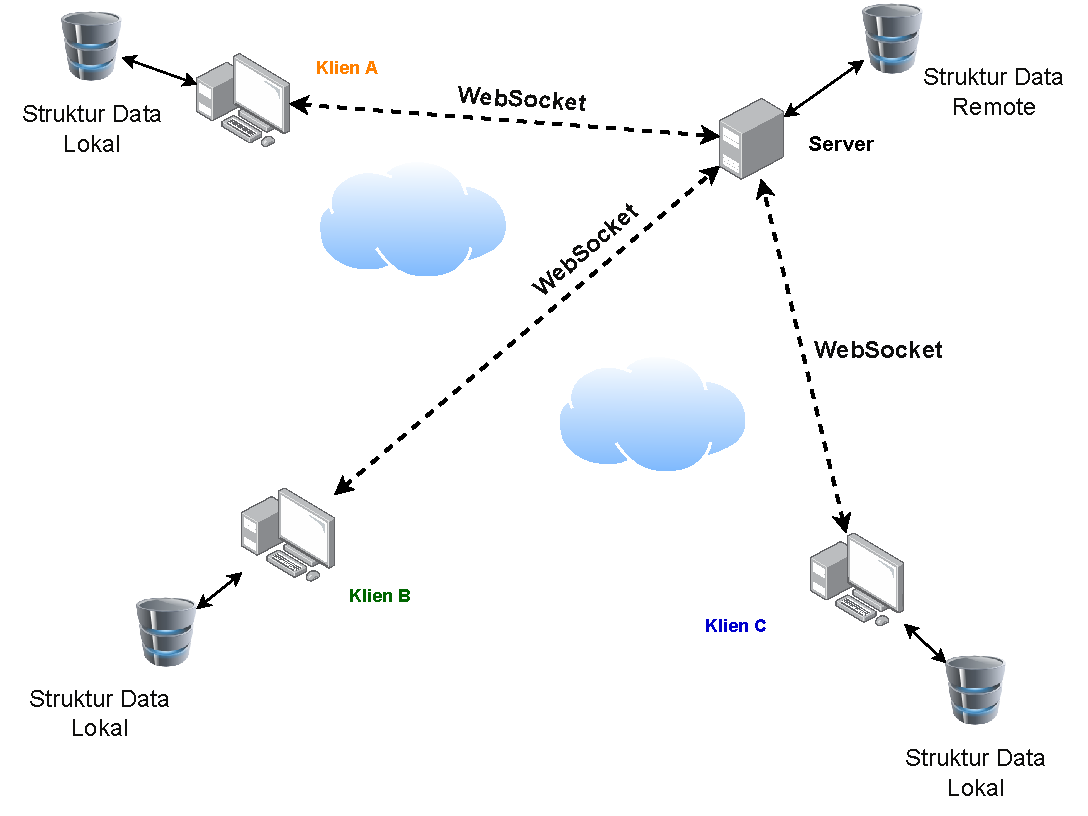
\includegraphics[scale=0.65]{assets/skripsi/Arsitektur_WebSocket_OT}
    \caption{Arsitektur yang Menggunakan WebSocket dan \textit{Operational Transformation}}
    \label{fig:websocket_ot}
\end{figure}

PeerToCP dengan variasi \textit{operational transformation} ini diilustrasikan pada gambar~\ref{fig:websocket_ot}. Pada kasus ini, Server tidak dapat menerima dua \textit{pending update} milik klien A sebelum ia memiliki semua versi terbaru dari server. Setelah melakukan \textit{pull update} dan menerima tiga operasi perubahan dari server, klien A akan mentransformasikan dua \textit{pending update}-nya dengan suatu algoritma \textit{operational transformation} terhadap tiga operasi baru ini. Kemudian klien A memperbaharui versi dokumen lokalnya menjadi versi 4, dan dapat mengirimkan \textit{update}-nya. Server selanjutnya akan menambahkan dua operasi dari klien A tersebut serta menjadikan server memiliki versi 6.

Hal yang serupa diterapkan juga untuk \textit{shell} program yang berjalan. Saat suatu klien memberikan \textit{keystroke} pada salah satu \textit{shell} yang aktif, \textit{keystroke} akan dikirimkan melalui mekanisme yang serupa, namun akan diarahkan ke klien yang menjadi \textit{host} atau menjalankan programnya. Selanjutnya, perubahan \textit{shell} akan dikirimkan berkala pada server selama ada perubahan yang belum diterima atau diketahui server. Saat terjadi perubahan, server akan melakukan pengumuman kepada setiap klien untuk melakukan \textit{pull}. Karena respons \textit{shell} bergantung pada klien \textit{host}, maka pembaharuan tidak perlu diterapkan fungsi transformasi seperti pada OT teks biasa. Salah satu aspek lainnya ialah \textit{position mapping} yang tidak perlu ditangani karena kursor akan selalu berada di sebelah kanan karakter terakhir. Operasi seperti mekanisme \textit{update} yang dilaksanakan secara serial ini diterapkan untuk mencegah terjadinya \textit{race condition} pada saat gangguan jaringan.

Beragam arsitektur yang sudah dipaparkan pada subbab-subbab sebelummya merupakan bagian \textit{backend} dari suatu antarmuka editor yang sama, sehingga penilaian secara \textit{end-to-end} yang akan dirasakan oleh pengguna menjadi tolok ukur yang logis dalam penelitian ini. Tolok ukur ini terdiri dari kasus yang mempertimbangkan aspek-aspek yang hendak diuji. Evaluasi dilakukan dengan perlakuan kontrol yang diusahakan identik untuk dapat memberikan hasil yang akurat.

\section{Desain Evaluasi}
\label{sec:desain_evaluasi}

Evaluasi sistem dilakukan dengan layanan Compute Engine Google Cloud Platform. Setiap variasi memiliki server yang di-\textit{deploy} pada \textit{instance} dengan zona daerah \texttt{asia-southeast1-b}, menggunakan mesin bertipe \texttt{e2-medium} yang memiliki 2 vCPUs dan memori RAM 4 GiB, serta sistem operasi Debian 11. Alasan dipilihnya mesin dengan tipe ini adalah untuk menghindari proses \textit{benchmarking} atau tolok ukur yang dibatasi oleh spesifikasi sistem. Dalam penelitian ini, \textit{relay server} tidak disediakan untuk \textit{peer} yang tidak dapat terhubung satu sama lain dalam sebuah jaringan \textit{peer-to-peer} berbasis WebRTC. Penelitian ini mengasumsikan inisialisasi koneksi \textit{peer-to-peer} WebRTC selalu berhasil pada variasi ini.

Untuk \textit{instance virtual machine} yang mewakili pengguna, digunakan mesin bertipe \texttt{e2-small} yang memiliki 2 vCPUs, memori Ram 2 GiB, dan sistem operasi Debian 11. Mesin pengguna akan di-\textit{deploy} pada \textit{zone} \texttt{asia-southeast2-a}. Setiap mesin pengguna diletakkan pada \textit{zone} yang sama, dan dekat dekat dengan server dengan tujuan untuk mensimulasikan perkiraan penggunaan aplikasi PeerToCP di dunia nyata. Terdapat empat skenario uji yang akan dilakukan terhadap sistem aplikasi. Skenario pertama secara praktis menyimulasikan serangkaian operasi-operasi tertentu terhadap editor teks dengan jumlah \textit{peer} sebanyak $n$ yang berbeda-beda. Jumlah klien atau \textit{peer} yang berbeda bertujuan untuk mewakilkan aspek \textit{scalability}. Terdapat tiga macam operasi acak yang dilakukan sebanyak sepuluh operasi per detik dalam periode uji tiga menit, yaitu:

\begin{enumerate}[nolistsep]
    \item memasukkan (\texttt{insert}) suatu \textit{string} karakter ASCII acak dengan panjang antara 2 hingga 5 secara inklusif;
    \item menghapus (\texttt{delete}) suatu \textit{range} dengan panjang antara 1 hingga 3 secara inklusif;
    \item menimpa (\texttt{replace}) suatu \textit{range} dengan panjang antara 2 hingga 5 dengan \textit{string} karakter ASCII acak dengan jangkauan yang sama.
\end{enumerate}

Operasi-operasi tersebut memiliki rata-rata penambahan sebanyak 15 karakter per detik dan perubahan sebanyak 41.67 karakter per detik (termasuk penghapusan) pada setiap kliennya. Tes dimulai bersamaan menggunakan \textit{timer} bawaan sistem operasi yang secara \textit{default} sudah disinkronisasi. Galat atau \textit{error} yang terdapat pada sinkronisasi waktu \textit{timer} tentunya tidak dapat dihindari, sehingga dianggap tidak ada. Namun, penelitian ini akan menggunakan \textit{instance} yang sama untuk setiap \textit{peer} atau kliennya sehingga mengurangi bias perbedaan \textit{timer} pada setiap klien dalam jaringan. Selain itu, akan ada operasi pemutusan jaringan (\textit{disconnect}) yang akan terjadi secara acak selama 30 detik di antara satu menit setelah uji skenario dimulai hingga satu menit sebelum uji skenario berakhir. Keadaan akhir editor teks setelah selesai akan sehendaknya terhubung ke server untuk melakukan sinkronisasi terakhir dengan \textit{peer-peer} lain dari server. Selama editor teks tidak terhubung, operasi-operasi lain seperti \texttt{insert}, \texttt{delete}, dan \texttt{replace} masih berjalan pada editor guna menggambarkan aspek \textit{local-first}.

Skenario pertama disusun selayaknya \textit{stress-testing} terhadap operasi-operasi editor teks yang dapat terjadi di dunia nyata. Di akhir tes, sistem menunggu selama satu menit untuk memberikan kelonggaran sinkronisasi. Waktu terakhir \textit{update} atau sinkronisasi akan disimpan untuk dibandingkan pada aspek \textit{responsiveness} dan \textit{scalability}. Nilai cacahan atau \textit{hash} dari dokumen setelah uji skenario juga turut dicatat pada setiap klien atau \textit{peer} serta dibandingkan satu sama lain untuk memenuhi aspek \textit{correctness}. Selain itu, aktivitas RAM, CPU, dan transmisi data dalam jaringan pada setiap klien beserta server akan direkam menggunakan \textit{framework} NetData untuk memenuhi aspek \textit{lightweight} dan \textit{scalability}.

Skenario kedua menggunakan \textit{environment} yang sama dengan skenario sebelumnya. Skenario ini disusun untuk menguji \textit{shell} pada setiap $n$ klien berbeda, yaitu dengan menjalankan suatu program C++ yang akan mencetak 100 bilangan tak bertanda (unsigned) 64-bit acak dengan jeda acak setiap bilangannya selama 500 hingga 1500 milidetik. Selama itu, akan dilakukan operasi pemutusan jaringan  \caption{Statistik Latensi Operasi Nonlokal pada Skenario Keempat (\textit{Shell} Bersama) dalam Satuan ms}
 (\textit{disconnect}) yang akan terjadi secara acak selama 20 detik setelah 10 hingga 40 detik setelah program berjalan. Seperti skenario sebelumnya, waktu sinkronisasi terakhir, aktivitas perangkat, dan nilai cacahan dari setiap \textit{shell} pada setiap klien akan dicatat dan dibandingkan untuk memastikan bahwa setiap pengguna memiliki replika \textit{shell} yang sama.

Skenario ketiga dan terakhir berpusat untuk mengukur latensi dari editor teks dan \textit{shell}. Pada skenario ketiga, $n$ peer disusun serupa dengan dua skenario sebelumnya. Terdapat dua operasi yang akan dilakukan, yaitu memasukkan (\texttt{insert}) \textit{timestamp} pada editor teks dan menimpa (\texttt{replace}) suatu \textit{range} dengan panjang antara 10 hingga 15 karakter dengan \textit{timestamp}. Setiap operasi yang dilakukan memiliki jeda acak selama 500 hingga 1000 milidetik guna menghindari operasi yang dilakukan secara bersamaan dalam periode yang tetap. Setiap klien atau \textit{peer} kemudian menangkap \textit{timestamp} dan mengukur latensi perbedaan saat \textit{timestamp} dicetak dan \textit{timestamp} diterima pada klien lainnya. Pada skenario keempat, setiap klien akan menjalankan program C++ yang akan mencetak 100 \textit{timestamp} dengan jeda acak selama 500 hingga 1500 milidetik. Setiap klien kemudian menangkap setiap \textit{event} ini dan mengukur latensinya dengan cara serupa, yaitu dengan menghitung selisih pemasukan konten timestamp oleh sebuah \textit{shell host} (pengguna yang menjalankan program) dengan penerimaan pada setiap pengguna lainnya. Pada skenario ketiga dan keempat ini, tidak ada operasi pemutusan pengguna dengan tujuan menghasilkan data yang akan dievaluasi pada aspek \textit{responsiveness} yang lebih akurat.
\clearchapter
%-----------------------------------------------------------------------------%
\chapter{\babLima}
\label{bab:5}

Bab ini membahas mengenai hasil dan analisis dari evaluasi yang telah dilaksanakan berdasarkan skenario-skenario yang telah disusun pada bab sebelumnya. Pembahasan analisis dibagikan berdasarkan aspek-aspek yang telah disusun untuk memberikan gambaran yang lebih jelas mengenai performa program dan penggunaan \textit{resource} atau sumber daya yang dibutuhkan untuk mencapai performa tersebut. Selain itu, bab ini juga membahas pertimbangan variasi dari PeerToCP yang lebih baik digunakan dan faktor-faktor yang memengaruhi pertimbangan tersebut. Melalui pertimbangan tersebut, kelemahan dari sistem aplikasi turut disampaikan untuk perkembangan ke depannya.

\section{Aspek \textit{Local-First} dan \textit{Correctness}}

Kedua aspek ini tidak dapat dipisahkan satu sama lain. Pada skenario pertama dan kedua, aspek \textit{local-first} diuji dengan menyimulasikan proses pemutusan koneksi secara acak pada klien sementara pengubahan data terus terjadi pada setiap pengguna lokal secara luring. Berdasarkan eksperimen secara langsung, proses perubahan ini terjadi secara \textit{local-first}, yang berarti perubahan lokal dapat terus dilakukan dan langsung diterapkan meskipun klien sedang tidak berada dalam jaringan. Ketika terjadi proses masuk kembali ke jaringan, data akan diperbaharui secara sesuai dengan perubahan yang dilakukan.

Berdasarkan eksperimen yang dilakukan, setiap variasi dari PeerToCP menghasilkan nilai hasil \textit{hash} atau cacahan yang sama untuk setiap skenarionya, yang berarti setiap dokumen berada pada kondisi atau \textit{state} akhir yang sama. Namun pada eksperimen yang dilakukan dalam skenario pertama dengan delapan klien variasi \textit{operational transformation} berbasis \textit{client-server}, terjadi pemutusan hubungan \textit{disconnection} yang tidak dapat terhubung kembali. Diperkirakan hal ini terjadi karena ketidakefektifan metode transmisi data pada PeerToCP variasi ini dan menyebabkan kebutuhan \textit{bandwidth} koneksi internet berada di luar batas \textit{environment} pengujian.

Skenario pertama variasi ini dengan jumlah klien delapan dilakukan pengulangan hingga tiga kali eksperimen. Dalam setiap eksperimen tersebut, satu hingga dua klien tidak dapat terhubung kembali. Pada eksperimen, waktu pemutusan hubungan dilakukan secara acak dalam periode durasi yang sama untuk setiap kliennya seperti yang dijelaskan pada bab sebelumnya. Grafik lebih detail yang menyatakan transmisi data masuk melalui jaringan pada klien pertama dan klien kedua untuk setiap variasi aplikasi dalam skenario pertama ini ditunukkan pada gambar grafik~ref{fig:2-23}.

\begin{figure}
 \centering
 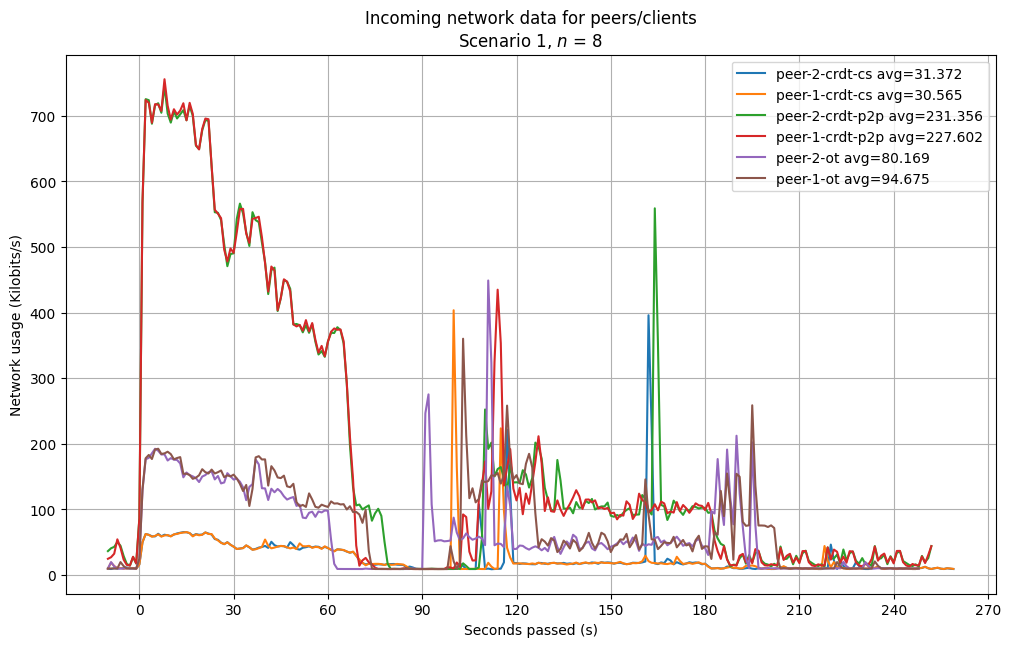
\includegraphics[width=13cm]{./assets/skripsi/benchmark-vis_cell_2_output_23}
 \caption{Grafik Perbandingan Jaringan pada Klien Pertama dan Klien Kedua untuk $n = 8$}
 \label{fig:2-23}
\end{figure}

Pada saat operasi \textit{update} dilakukan tepat setelah koneksi terhubung kembali, ukuran \textit{update} cenderung lebih besar karena sudah terkumpul dari beberapa operasi yang terjadi selama klien sedang berada di luar jaringan. Ketika \textit{update} ini dilakukan, server sedang dalam keadaan berbagai klien lain yang hendak mengirimkan \textit{update}. Karena hal tersebut, algoritma \textit{operational transformation} yang hanya membolehkan suatu \textit{update} untuk dilakukan apabila versi terbaru yang sama sudah dimiliki oleh klien akan meminta klien untuk melakukan \textit{update}. Sementara tumpukan \textit{push update} berukuran besar terus dikirimkan hal ini akan memenuhi \textit{bandwidth} server, yang dapat dilihat pada grafik berikut.

Gambar~\ref{fig:2-23}, menunjukkan klien pertama yang mengalami pemutusan jaringan pada detik ke-72 dan penghubungan kembali pada detik ke-102, terjadi pengiriman data yang cukup besar selama kurang lebih 20 detik. Begitu pula dengan klien kedua yang mengalami pemutusan jaringan pada sekitar detik ke-60 dan penghubungan kembali pada detik ke-90. Sesaat setelah suatu klien terhubung kembali ke suatu jaringan, terjadi \textit{spike} pada jaringan yang cukup besar. Pada jumlah pengguna yang cukup banyak dalam satu dokumen, pemutusan dan penghubungan jaringan yang secara sengaja dilakukan pada waktu yang serupa dapat menyebabkan ketidakandalan pada sistem ini. Grafik untuk server ditunjukkan pada gambar grafik~/ref{fig:2-24}.

\begin{figure}
 \centering
 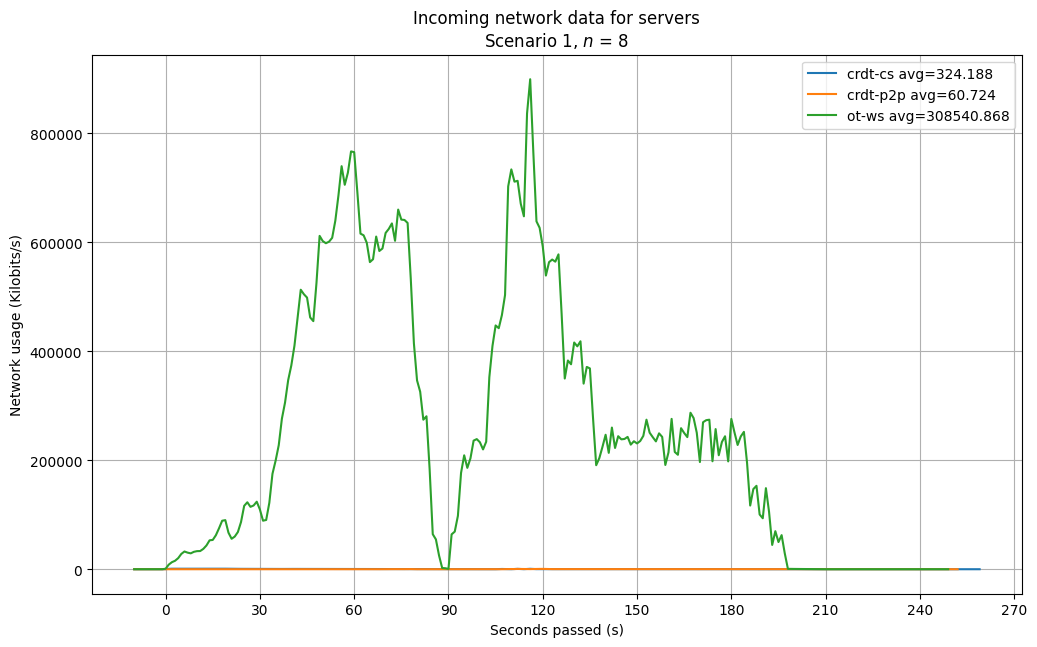
\includegraphics[width=15cm]{./assets/skripsi/benchmark-vis_cell_2_output_24}
 \caption{Grafik Perbandingan Penerimaan Data pada Setiap Variasi Server PeerToCP}
 \label{fig:2-24}
\end{figure}

Lalu lintas jaringan pada server variasi \textit{operational transformation} dengan arsitektur \textit{client-server} dapat mencapai lebih dari 800000 \textit{kilobits}/detik atau setara dengan 100 \textit{megabytes}/detik, sementara untuk skenario yang serupa, transmisi data pada server dengan variasi CRDT berarsitektur \textit{client-server} lebih hemat sekitar 950 kali. Melalui gambar~\ref{fig:2-24}, diketahui bahwa rata-rata transmisinya sekitar 80 kali lebih sedikit dibandingkan CRDT \textit{peer-to-peer} serta 950 kali lebih sedikit dibandingkan CRDT \textit{client-server}.

Pada skenario pertama ini, terlihat bahwa variasi PeerToCP yang menggunakan CRDT lebih dapat diandalkan karena paralelitas \textit{update} yang dilakukan terhadap dokumen. Faktor-faktor lain yang memengaruhi variasi CRDT yang lebih baik juga tidak menutup kemungkinan dari segi implementasi \textit{provider websocket} yang digunakan, teknik kompresi dan \textit{encoding} yang diterapkan, serta efek bola salju yang ditimbulkan akibat \textit{update} berukuran besar yang terus dikirimkan menjadi tertumpuk dan selalu terlambat dibandingkan \textit{update} lain dan menyangkut aspek selanjutnya, yaitu \textit{Scalability} dan \textit{Responsiveness}.

\section{Aspek \textit{Scalability} dan \textit{Responsiveness}}

Latensi dari teks editor secara khusus diukur secara terus-menerus pada skenario ketiga tanpa adanya pemutusan hubungan seperti pada skenario pertama dan kedua. Setiap pengguna diukur waktu selisih penerimaan datanya terhadap pengguna yang bukan dirinya sendiri dan dicatat latensinya pada waktu data dokumen diterima, kemudian dilakukan rata-rata untuk $n$ pengguna tersebut. Tabel~\ref{tab:latency-3} menunjukkan latensi PeerToCP variasi CRDT \textit{peer-to-peer} memiliki latensi yang paling rendah, namun semakin besar nilai $n$, selisih perbedaan CRDT \textit{client-server} dan CRDT \textit{peer-to-peer} semakin mengecil. Sementara pada variasi OT \textit{client-server}, latensinya dua kali lebih besar dari variasi CRDT \textit{client-server}, dengan lonjakan latensi maksimum hingga dua detik saat $n = 8$.

% Please add the following required packages to your document preamble:
% \usepackage{multirow}
\begin{table}[H]
 \centering
\begin{tabular}{|c|rrr|rrr|rrr|}
\hline
\multirow{2}{*}{$n$} & \multicolumn{3}{c|}{\textbf{CRDT \textit{Peer-To-Peer}}} & \multicolumn{3}{c|}{\textbf{CRDT \textit{Client-Server}}} & \multicolumn{3}{c|}{\textbf{OT \textit{Client-Server}}} \\ \cline{2-10}
 & \multicolumn{1}{c|}{Mean} & \multicolumn{1}{c|}{Median} & \multicolumn{1}{c|}{Max} & \multicolumn{1}{c|}{Rerata} & \multicolumn{1}{c|}{Median} & \multicolumn{1}{c|}{Max} & \multicolumn{1}{c|}{Rerata} & \multicolumn{1}{c|}{Median} & \multicolumn{1}{c|}{Max} \\ \hline
\textbf{2} & \multicolumn{1}{r|}{23.30} & \multicolumn{1}{r|}{21.00} & 76.00 & \multicolumn{1}{r|}{39.50} & \multicolumn{1}{r|}{38.00} & 134.00 & \multicolumn{1}{r|}{87.42} & \multicolumn{1}{r|}{84.00} & 168.00 \\ \hline
\textbf{4} & \multicolumn{1}{r|}{34.00} & \multicolumn{1}{r|}{30.00} & 223.00 & \multicolumn{1}{r|}{46.10} & \multicolumn{1}{r|}{42.00} & 220.00 & \multicolumn{1}{r|}{98.84} & \multicolumn{1}{r|}{86.00} & 1225.00 \\ \hline
\textbf{8} & \multicolumn{1}{r|}{55.56} & \multicolumn{1}{r|}{47.00} & 313.00 & \multicolumn{1}{r|}{63.84} & \multicolumn{1}{r|}{56.00} & 308.00 & \multicolumn{1}{r|}{235.62} & \multicolumn{1}{r|}{151.00} & 2010.00 \\ \hline
\end{tabular}
 \caption{Statistik Latensi Operasi Nonlokal pada Skenario Ketiga (Teks Editor Bersama) dalam ms}
 \label{tab:latency-3}
\end{table}

Dari segi skalabilitasnya, dengan asumsi pengguna berada dalam jarak yang dekat, misalnya dalam kasus ini setiap \textit{peers} berada dalam satu zona yang sama, yaitu Indonesia. Variasi \textit{peer-to-peer} memberikan performa yang optimal dibandingkan \textit{client-server} untuk jumlah $n$ tertentu. Berdasarkan perhitungan dan proyeksi jumlah pengguna yang bertambah, variasi dari CRDT \textit{client-server} dapat memberikan \textit{responsiveness} yang lebih baik untuk suatu nilai $n$ yang lebih tinggi atau saat \textit{peers} berada pada daerah yang lebih jauh antara satu sama lainnya.

Perbedaan latensi ini dapat disebabkan oleh faktor jaringan dan arsitekturnya atau algoritma yang memastikan bahwa dokumen tersebut sama pada setiap replikanya. Dari analisis algoritma, variasi CRDT memberikan latensi melakukan penerapan operasi lokal waktu yang sama. Operasi lokal dalam konteks ini ialahoperasi pada klien tersebut sendiri yang bersifat luring serta \textit{local-first}. dengan  Dalam praktisnya, gambar~\ref{fig:12-5} menunjukkan adanya perbedaan latensi yang tidak terlalu signifikan, yaitu dengan rata-rata sekitar 5ms. Perlu diketahui juga bahwa nilai lonjakan latensi maksimalnya yang berdekatan. Perlu diketahui bahwa skalabilitas latensi algoritma CRDT dan OT tumbuh secara berbeda. Kompleksitas waktu dari OT dipengaruhi oleh banyaknya \textit{update} berbeda, sementara kompleksitas waktu CRDT dipengaruhi oleh banyaknya karakter atau ukuran dokumen.

\begin{figure}
 \centering
 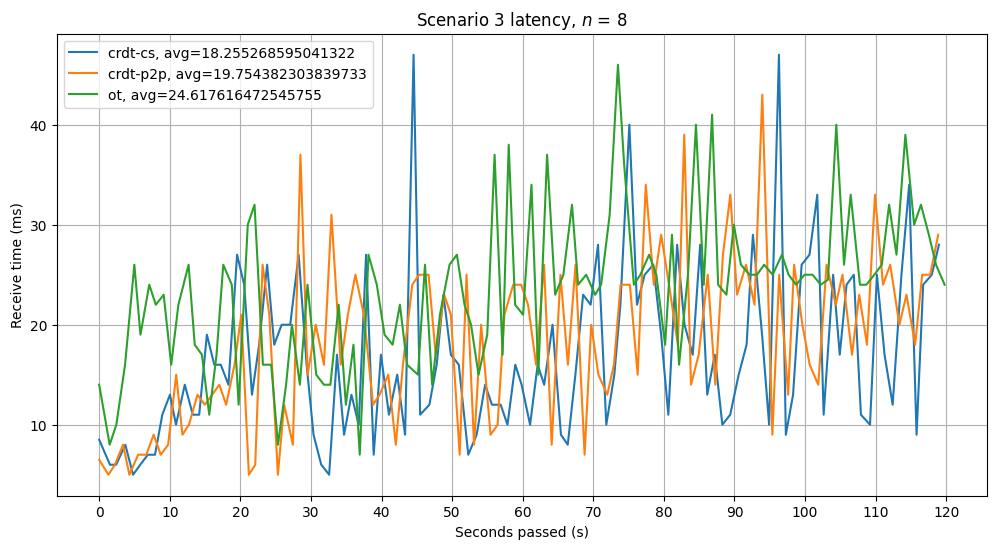
\includegraphics[width=15cm]{./assets/skripsi/benchmark-vis_cell_12_output_5}
 \caption{Grafik Waktu \textit{Resolve} Operasi Lokal pada Editor Setiap Variasi Aplikasi Pengguna PeerToCP}
 \label{fig:12-5}
\end{figure}

Latensi total diperoleh dari waktu penerapan operasi lokal dan nonlokal ditambah dengan waktu transmisi jaringan pada arsitektur yang berbeda-beda. Gambar~\ref{fig:7-5} menunjukkan perbedaan latensi yang cukup besar, serta lonjakan latensi yang terjadi beberapa kali sepanjang skenario ketiga berjalan. Hal ini dapat disebabkan oleh beberapa hal, yakni waktu \textit{resolve} operasi nonlokal dan adanya efek penumpukan \textit{update} yang diilustrasikan pada diagram gambar~\ref{diagram:snowball}.

\begin{figure}
 \centering
 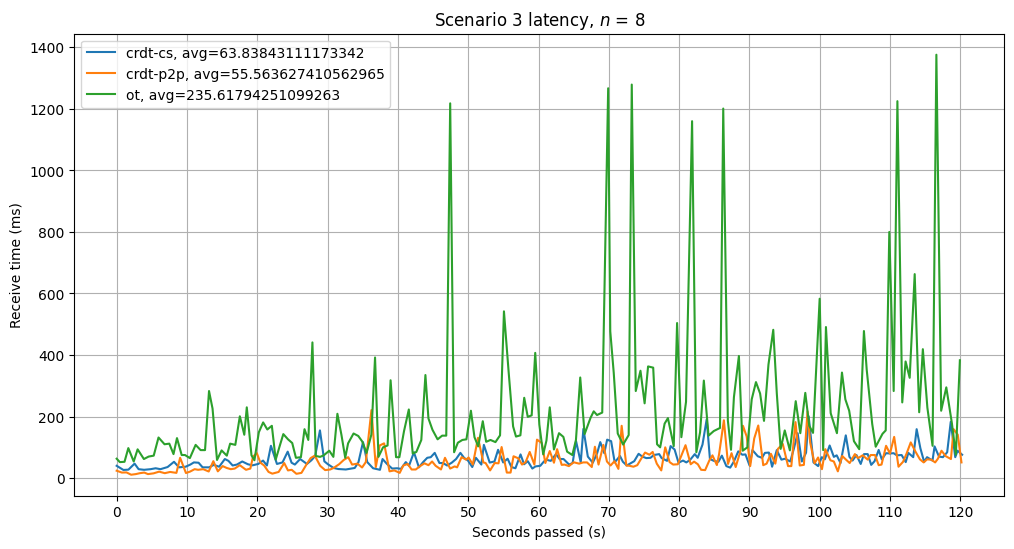
\includegraphics[width=15cm]{./assets/skripsi/benchmark-vis_cell_7_output_5}
 \caption{Grafik Rata-Rata Latensi pada Operasi Nonlokal Setiap Variasi Aplikasi Pengguna PeerToCP}
 \label{fig:7-5}
\end{figure}

\begin{figure}
 \centering
 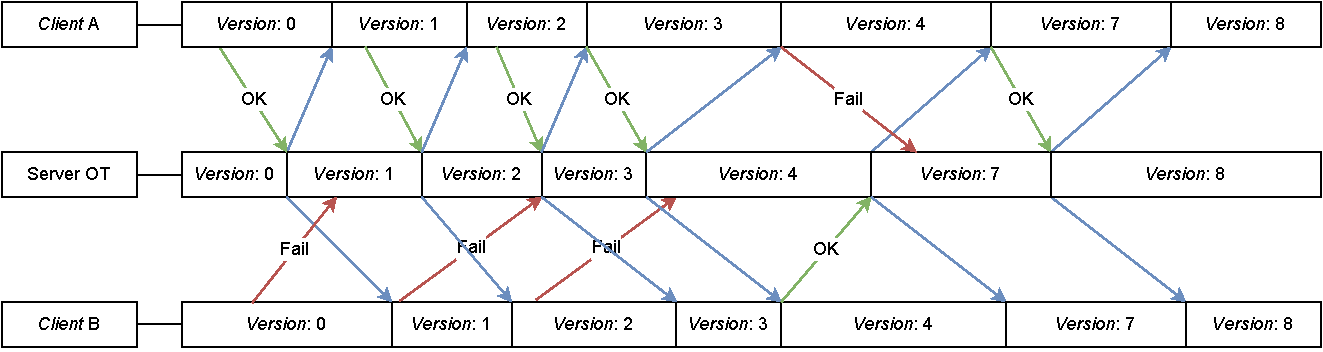
\includegraphics[width=15cm]{./assets/skripsi/Snowball}
 \caption{Diagram Ilustrasi Penumpukan \textit{Update}}
 \label{diagram:snowball}
\end{figure}

Pada arsitektur \textit{operational transformation} berbasis \textit{client-server}, \textit{update} dari suatu klien tidak akan diterima oleh server apabila klien tersebut belum memiliki versi terbaru dari server. Penumpukan \textit{update} ini dapat terjadi karena klien tersebut semakin tidak bisa mengirimkan datanya karena semakin besar dan selalu didahului oleh klien lain yang berada dalam jaringan tersebut. Penumpukan ini dapat menyebabkan tidak dapat diperbaruinya salah satu klien dan transmisi data keluar yang besar karena pengiriman \textit{update} besar yang dilakukan terus-menerus.

Dalam praktis penggunaan realistisnya, hal ini diperkirakan tidak umum terjadi karena frekuensi pengetikan atau pemasukan karakter tidak dilakukan secara bersamaan dan tidak sebanyak skenario pertama dan kedua. Operasi salin dan tempel secara berkali-kali dapat berpotensi menyebabkan hal ini terjadi karena perubahan dokumen dalam jumlah karakter yang banyak terjadi. Namun dalam praktisnya, operasi tersebut diasumsikan hanya dilakukan dengan jeda frekuensi yang membolehkan setiap klien dalam jaringan memperbarui replikanya sebelum operasi besar lain dilakukan.

Skenario empat menguji latensi \textit{shell} yang dapat digunakan secara bersama. Secara umum, latensi tersebut dideskripsikan pada tabel~\ref{tab:latency-4}. Berbeda halnya dengan \textit{editor teks} yang waktu penerapan operasinya berdampak sebesar 20--70ms atau lebih. Struktur data berupa \textit{dictionary} sederhana pada \textit{shell} tidak memberikan perbedaan yang signifikan seperti yang digambarkan pada gambar grafik~\ref{fig:13-5}.

% Please add the following required packages to your document preamble:
% \usepackage{multirow}
\begin{table}[H]
 \centering
\begin{tabular}{|c|rrr|rrr|rrr|}
\hline
\multirow{2}{*}{$n$} & \multicolumn{3}{c|}{\textbf{CRDT \textit{Peer-To-Peer}}} & \multicolumn{3}{c|}{\textbf{CRDT \textit{Client-Server}}} & \multicolumn{3}{c|}{\textbf{OT \textit{Client-Server}}} \\ \cline{2-10}
 & \multicolumn{1}{c|}{Mean} & \multicolumn{1}{c|}{Median} & \multicolumn{1}{c|}{Max} & \multicolumn{1}{c|}{Rerata} & \multicolumn{1}{c|}{Median} & \multicolumn{1}{c|}{Max} & \multicolumn{1}{c|}{Mean} & \multicolumn{1}{c|}{Median} & \multicolumn{1}{c|}{Max} \\ \hline
\textbf{2} & \multicolumn{1}{r|}{3.05} & \multicolumn{1}{r|}{3.00} & 5.00 & \multicolumn{1}{r|}{16.75} & \multicolumn{1}{r|}{17.00} & 19.00 & \multicolumn{1}{r|}{31.79} & \multicolumn{1}{r|}{30.00} & 170.00 \\ \hline
\textbf{4} & \multicolumn{1}{r|}{3.13} & \multicolumn{1}{r|}{3.00} & 6.00 & \multicolumn{1}{r|}{16.55} & \multicolumn{1}{r|}{17.00} & 21.00 & \multicolumn{1}{r|}{44.47} & \multicolumn{1}{r|}{32.00} & 309.00 \\ \hline
\textbf{8} & \multicolumn{1}{r|}{3.36} & \multicolumn{1}{r|}{3.00} & 19.00 & \multicolumn{1}{r|}{17.16} & \multicolumn{1}{r|}{17.00} & 35.00 & \multicolumn{1}{r|}{59.86} & \multicolumn{1}{r|}{30.33} & 551.00 \\ \hline
\end{tabular}
 \caption{Statistik Latensi Operasi Nonlokal pada Skenario Keempat (\textit{Shell} Bersama) dalam Satuan ms}
 \label{tab:latency-4}
\end{table}

\begin{figure}
 \centering
 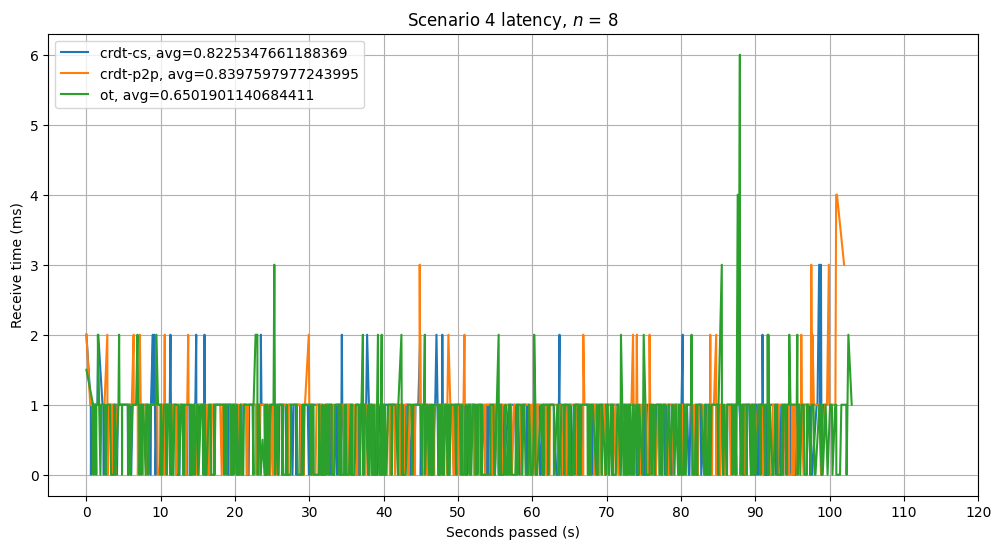
\includegraphics[width=15cm]{./assets/skripsi/benchmark-vis_cell_13_output_5}
 \caption{Grafik Waktu \textit{Resolve} Operasi Lokal pada \textit{Shell} Setiap Variasi Aplikasi Pengguna PeerToCP}
 \label{fig:13-5}
\end{figure}

Hal ini dikarenakan operasi penerapan dari \textit{append-only array} pada \textit{operational transformation} memiliki kompleksitas waktu konstan secara \textit{amortized}. Sehingga secara skalabilitas, hanya berpengaruh terhadap efektivitas dan performa latensi dari transmisi data, yang mengalami permasalahan sama seperti pada skenario pertama, kedua, dan ketiga seperti yang ditunjukkan pada gambar grafik~\ref{fig:9-5}. Faktor lain yang mempengaruhi alasan latensi \textit{operational transformation} lebih lambat dari pada CRDT \textit{client-server} ialah mekanisme komunikasinya. Implementasi CRDT Yjs dilengkapi dengan proses \textit{encoding} dan \textit{decoding} yang membuat transmisinya dalam jaringan untuk data yang besar dapat lebih cepat, serta tidak diperlukan adanya operasi \textit{update} yang dilakukan secara berurutan. Sementara implementasi variasi \textit{operational transformation}-nya masih menggunakan mekanisme \textit{update} yang sama dengan \textit{editor teks}-nya, hanya dengan perbedaan kompleksitas waktu \textit{update} konstan \textit{shell}.

\begin{figure}
 \centering
 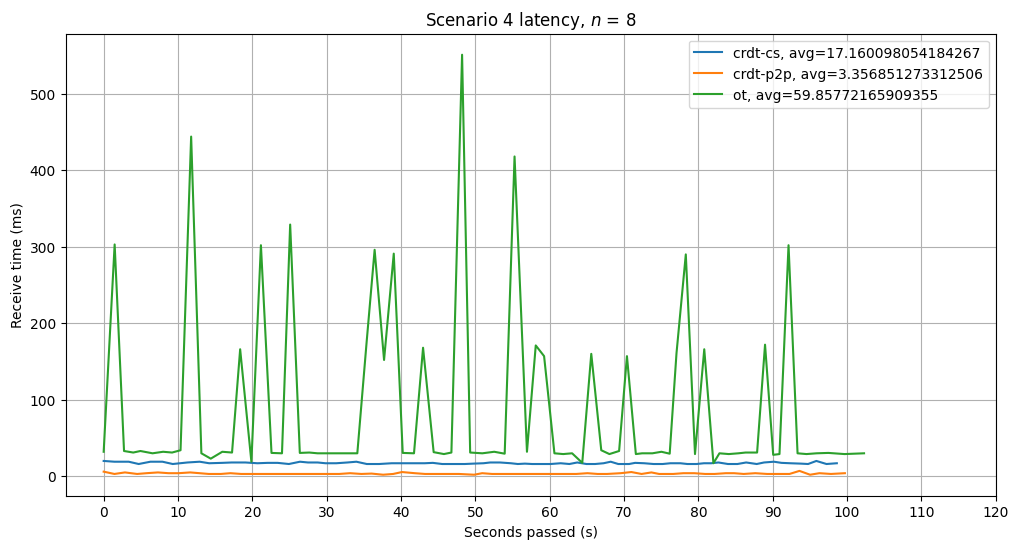
\includegraphics[width=15cm]{./assets/skripsi/benchmark-vis_cell_9_output_5}
 \caption{Grafik Rata-Rata Latensi pada Operasi Nonlokal Setiap Variasi Aplikasi Pengguna PeerToCP}
 \label{fig:9-5}
\end{figure}

Bila dibandingkan dengan arsitektur \textit{peer-to-peer}, setiap \textit{peers} dalam jaringan tersebut berada dalam jarak yang cenderung dekat. Latensinya akan lebih rendah dibandingkan kedua arsitektur \textit{client-server} yang harus melewati server terlebih dahulu. Secara umum, variasi yang terbaik ialah variasi CRDT dengan arsitektur \textit{peer-to-peer} sejumlah $n$ tertentu. Dalam konteks eksperimen ini, untuk $n \leq 8$, variasi \textit{peer-to-peer} masih memberikan performa terbaik dari setiap variasi lainnya dari aspek \textit{responsiveness}. Diperkirakan untuk suatu nilai $n > 8$, atau jarak antar \textit{peers} yang lebih jauh, variasi CRDT dengan arsitektur \textit{client-server} dapat dipertimbangkan sebagai alternatif. Dalam beberapa kasus lainnya, CRDT \textit{peer-to-peer} dengan WebRTC dapat mengalami permasalahan antar \textit{peers} yang tidak dapat saling terhubung. Sehingga, alternatif berupa server penghubung, \textit{relay} atau STUN dapat digunakan dan latensinya memerlukan eksperimen lebih lanjut untuk dapat dibandingkan. Variasi \textit{operational transformation} juga dapat dipertimbangkan, karena secara teori operasi \textit{update}-nya yang konstan dapat memberikan latensi yang lebih baik karena memanfaatkan sifat \textit{append-only array} dan hanya satu \textit{peer} atau klien yang bertanggung jawab untuk meneruskan data interaksinya pada suatu \textit{shell}.

Untuk mendapatkan latensi yang optimal, struktur data CRDT dapat dimodifikasi dengan memanfaatkan sifat tersebut. Lebih lanjut, sistem dapat dimodifikasi untuk menentukan arsitektur optimal antara \textit{peer-to-peer} tanpa \textit{relay server} seperti pada eksperimen ini, \textit{peer-to-peer} dengan \textit{relay server} untuk menangani \textit{peer} yang tidak dapat terhubung oleh WebRTC, atau pun \textit{client-server} apabila banyaknya pengguna atau \textit{peer} dalam jaringan cukup banyak. Dari segi latensi, pertimbangan hal tersebut dapat ditentukan dengan metriks sederhana seperti \textit{ping} antarpengguna yang dilakukan dari layar belakang aplikasi. Namun, dalam praktisnya terdapat beberapa faktor lain yang harus dipertimbangkan, yakni berupa sifat \textit{lightweight} atau sebarapa banyak proses atau pekerjaan, serta memori yang harus disediakan oleh server dan penggunanya.

\section{Aspek \textit{Lightweight}}

Aspek ini memaparkan seberapa besar \textit{resource} komputasi yang dibutuhkan untuk setiap \textit{peers} dan servernya. Semua metriks RAM diukur dengan melakukan normalisasi ke nol sesaat sebelum uji kasus dimulai. Pengukuran ini didasarkan untuk membandingkan perubahan pertumbuhan. Selain itu, dalam beberapa kasus dalam menjalankan klien, aplikasi elektron yang berjalan di atas Chromium memiliki sistem \textit{garbage collection} dan \textit{cache}~\citep{chromium}. Sehingga, pengukuran skenario yang dilakukan relatif terhadap ukuran memori sesaat sebelum tes dimulai untuk memberikan perbandingan pertumbuhan yang lebih jelas. Pada mulanya, setiap server mulai dengan RAM yang relatif rendah, yakni di bawah 20MiB. Sementara setiap peers mulai dengan RAM yang cenderung lebih tinggi, yakni sekitar 200 MiB. Aplikasi ini membutuhkan memori yang cukup besar karena menggunakan \textit{framework} Electron yang menjalankan peramban web Chromium pada \textit{front-end}-nya.

\begin{table}[H]
 \centering

\begin{tabular}{|cc|r|r|r|}
\hline
\multicolumn{2}{|c|}{$n$} & \multicolumn{1}{c|}{\textbf{2}} & \multicolumn{1}{c|}{\textbf{4}} & \multicolumn{1}{c|}{\textbf{8}} \\ \hline
\multicolumn{1}{|c|}{\multirow{4}{*}{\textbf{CRDT \textit{Peer-To-Peer}}}} & CPU & 39.1964893 & 60.13947488 & 62.2870496 \\ \cline{2-5}
\multicolumn{1}{|c|}{} & RAM & 16.57856816 & 19.24442935 & 21.30499303 \\ \cline{2-5}
\multicolumn{1}{|c|}{} & Net In & 28.5230253 & 96.16536701 & 229.4788353 \\ \cline{2-5}
\multicolumn{1}{|c|}{} & Net Out & -28.03809012 & -93.97903876 & -223.6266535 \\ \hline
\multicolumn{1}{|c|}{\multirow{4}{*}{\textbf{CRDT \textit{Client-Server}}}} & CPU & 33.96390498 & 57.38616741 & 56.89049428 \\ \cline{2-5}
\multicolumn{1}{|c|}{} & RAM & 14.92823532 & 19.12934751 & 20.94699478 \\ \cline{2-5}
\multicolumn{1}{|c|}{} & Net In & 19.46582482 & 27.68880062 & 30.96869733 \\ \cline{2-5}
\multicolumn{1}{|c|}{} & Net Out & -19.76281471 & -21.21326889 & -18.73440885 \\ \hline
\multicolumn{1}{|c|}{\multirow{4}{*}{\textbf{OT \textit{Client-Server}}}} & CPU & 47.79374975 & 73.29454876 & 65.25737338 \\ \cline{2-5}
\multicolumn{1}{|c|}{} & RAM & 25.9460194 & 31.17265199 & 36.33549154 \\ \cline{2-5}
\multicolumn{1}{|c|}{} & Net In & 62.24127487 & 99.81376692 & 87.42216719 \\ \cline{2-5}
\multicolumn{1}{|c|}{} & Net Out & -12962.04576 & -28872.47276 & -18344.14905 \\ \hline
\end{tabular}
 \label{tab:resource-client-1}
 \caption{Statistik Rata-Rata Aktivitas dan \textit{Resource} Aplikasi Pengguna pada Skenario Pertama}
\end{table}

Tabel~\ref{tab:resource-client-1} berturut-turut memiliki parameter yang menunjukkan aktivitas utilitasi CPU dalam satuan persen utilisasi, 100\% utilisasi berarti sistem menggunakan satu \textit{core} vCPU dengan penuh. Selanjutnya sumber daya atau resource RAM yang sudah dinormalisasi dalam satuan MiB, diikuti dengan kecepatan penerimaan dan pengiriman data dalam satuan kilobits per detik. Penggunaan RAM dan penerimaan data pada variasi CRDT \textit{peer-to-peer} cenderung lebih tinggi untuk $n = 8$, hal ini disebabkan karena pada variasi ini, semakin banyak \textit{peers} pada jaringan, berarti semakin banyak pula replika dokumen yang harus disinkronisasi. Karena \textit{signalling server} pada variasi ini tidak berperan dalam transmisi data CRDT, sehingga setiap \textit{peers} bertanggung jawab untuk saling memberikan informasi satu sama lain dalam memastikan kesamaan informasi pada setiap replikanya. Dari segi banyaknya data yang masuk ke dalam aplikasi variasi CRDT memastikan bahwa data-data tersebut dapat digunakan secara langsung dan setiap data yang dikirimkan akan digunakan tanpa ada kasus penolakan \textit{update} seperti pada variasi OT. Sehingga dari segi transmisi data keluar, variasi CRDT dianggap jauh lebih memenuhi aspek \textit{lightweight} dibandingkan variasi OT.

Variasi aplikasi CRDT \textit{client-server} secara relatif memberikan performa yang lebih baik untuk setiap variasi dari PeerToCP. Dari segi utilisasi CPU pada \textit{environment} pengujian dengan dua core vCPU (utilisasi maksimal 200\%), skenario pertama dengan $n \geq 4$ secara rata-rata hanya menggunakan sekitar 1/3 \textit{resource} dari CPU seperti yang terlihat pada gambar grafik~\ref{fig:2-19}. Metriks ini dapat dipertimbangkan dengan tambahan bahwa skenario ini memberikan muatan operasi-operasi yang relatif lebih besar dan banyak dari perkiraan aktivitas penggunaan normal. Selain itu, sistem operasi secara optimal akan menentukan proses yang harus diutamakan baik dari segi penyimpanan dan prioritas komputasi saat berjalannya aplikasi-aplikasi di atas sistem.

\begin{figure}
 \centering
 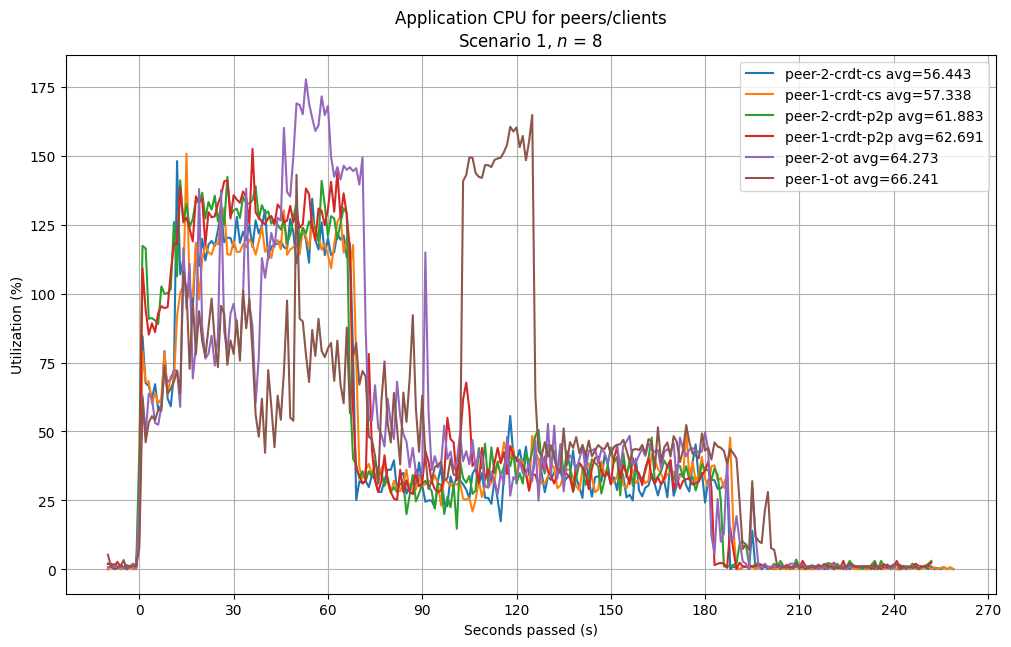
\includegraphics[width=13cm]{./assets/skripsi/benchmark-vis_cell_2_output_19}
 \caption{Grafik Perbandingan Utilisasi CPU pada Klien Pertama dan Klien Kedua untuk $n = 8$}
 \label{fig:2-19}
\end{figure}

\begin{figure}
 \centering
 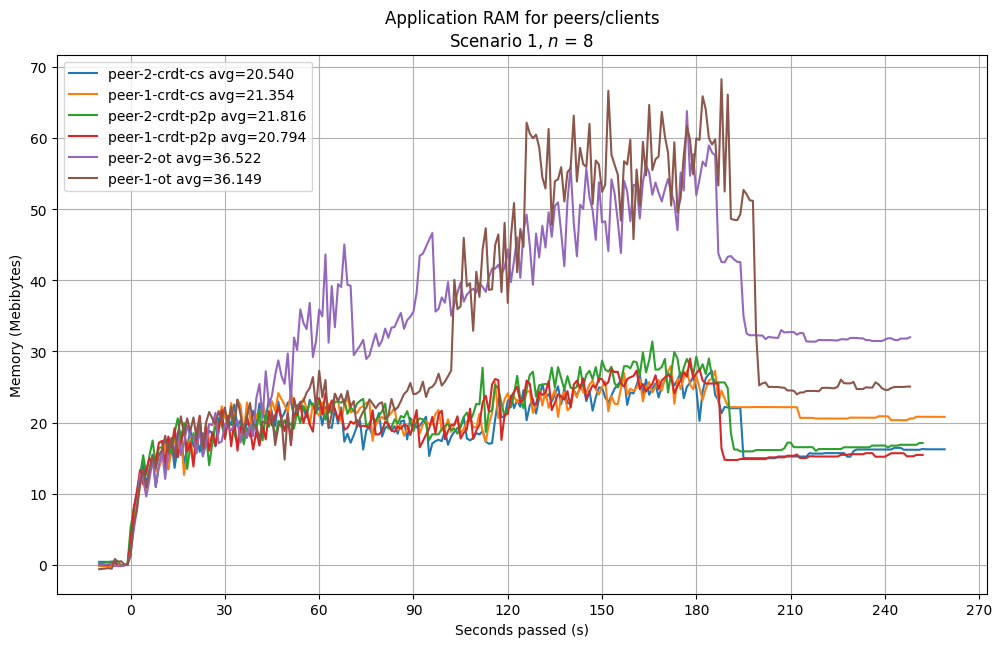
\includegraphics[width=13cm]{./assets/skripsi/benchmark-vis_cell_2_output_21}
 \caption{Grafik Perbandingan Penggunaan RAM pada Klien Pertama dan Klien Kedua untuk $n = 8$}
 \label{fig:2-21}
\end{figure}

Dari segi memori, kedua variasi CRDT memberikan pertumbuhan yang lebih optimal dibandingkan variasi OT. Namun, setiap variasinya menggunakan memori yang relatif kecil terhadap kapasitas penuh perangkat \textit{environment} pengujian, yakni sekitar 15\%. Penggunaan memori sebelum dinormalisasi rata-rata dimulai dengan menggunakan sekitar 200MiB, diikuti dengan pertumbuhan penggunaan seperti yang terlihat pada gambar grafik~\ref{fig:2-21}. Sistem operasi dapat memanfaatkan CPU dan RAM yang \textit{idle} sehingga utilisasinya dapat mendominasi proses lain pada komputer. Selama aplikasi tidak menggunakan utilisasi penuh yang mengganggu jalannya aktivitas pengguna dalam berinteraksi dengan aplikasi PeerToCP dan aplikasi lain, maka penggunaannya untuk jumlah pengguna yang terbatas dan diuji dalam eksperimen bagi pengguna setiap variasi PeerToCP dianggap memenuhi aspek \textit{lightweight} dari segi utilisasi CPU dan RAM.


\begin{table}[H]
 \centering
\begin{tabular}{|cc|r|r|r|}
\hline
\multicolumn{2}{|c|}{$\boldsymbol{n}$} & \multicolumn{1}{c|}{\textbf{2}} & \multicolumn{1}{c|}{\textbf{4}} & \multicolumn{1}{c|}{\textbf{8}} \\ \hline
\multicolumn{1}{|c|}{\multirow{4}{*}{\textbf{CRDT \textit{Peer-To-Peer}}}} & CPU & 0.01 & 0.02 & 0.10 \\ \cline{2-5}
\multicolumn{1}{|c|}{} & RAM & 0.67 & -0.03 & 0.40 \\ \cline{2-5}
\multicolumn{1}{|c|}{} & Net In & 10.72 & 14.81 & 60.72 \\ \cline{2-5}
\multicolumn{1}{|c|}{} & Net Out & -10.24 & -15.79 & -83.11 \\ \hline
\multicolumn{1}{|c|}{\multirow{4}{*}{\textbf{CRDT \textit{Client-Server}}}} & CPU & 0.93 & 1.29 & 1.68 \\ \cline{2-5}
\multicolumn{1}{|c|}{} & RAM & 5.01 & 6.83 & 9.54 \\ \cline{2-5}
\multicolumn{1}{|c|}{} & Net In & 73.26 & 176.64 & 324.19 \\ \cline{2-5}
\multicolumn{1}{|c|}{} & Net Out & -71.79 & -193.90 & -391.66 \\ \hline
\multicolumn{1}{|c|}{\multirow{4}{*}{\textbf{OT \textit{Client-Server}}}} & CPU & 4.85 & 14.18 & 24.33 \\ \cline{2-5}
\multicolumn{1}{|c|}{} & RAM & 30.92 & 41.88 & 69.99 \\ \cline{2-5}
\multicolumn{1}{|c|}{} & Net In & 52318.08 & 167768.04 & 308540.87 \\ \cline{2-5}
\multicolumn{1}{|c|}{} & Net Out & -26494.76 & -84932.31 & -156178.28 \\ \hline
\end{tabular}
 \caption{Statistik Rata-Rata Aktivitas dan \textit{Resource Server} pada Skenario Pertama}
 \label{tab:resource-server-1}
\end{table}

Aspek \textit{lightweight} lainnya yang perlu dipertimbangkan ialah penggunaan \textit{resource} atau sumber daya pada server yang dideskripsikan pada tabel~\ref{tab:resource-server-1}. Server CRDT \textit{peer-to-peer} yang akan menyelesaikan \textit{signalling} WebRTC menggunakan \textit{resource} RAM dan CPU yang sangat minim, dan secara teori tidak mengalami perbedaan signifikan untuk suatu jaringan yang sedang menggunakan aplikasi ini, karena hanya menangani klien yang masuk dan keluar pada suatu kelompok \textit{peer}. Berbeda halnya dengan arsitektur \textit{client-server}, selain berperan dalam memelihara koneksi kelompok klien dalam suatu ruangan, server juga memelihara kondisi replika pada setiap klien dalam jaringan. Dalam beberapa referensi implementasi, penyimpanan dokumen dapat memerlukan basis data yang lebih besar untuk dapat menampung lebih banyak data pada kelompok jaringan. Dalam eksperimen ini, basis data pada setiap variasi tidak menggunakan teknologi pihak ketiga dan hanya menggunakan struktur data bawaan sederhana pada server.

Dari data statistik tersebut, \textit{drawback} dari transmisi minimal pada aplikasi pengguna CRDT \textit{client-server} ialah transmisi yang lebih besar dari sisi server, dan sebaliknya pada CRDT \textit{peer-to-peer}, transmisi data cenderung lebih kecil dibandingkan dengan variasi \textit{peer-to-peer}nya. Variasi OT memiliki muatan paling besar dibandingkan dengan variasi lain yang juga secara tidak langsung memengaruhi utilisasi \textit{resource}-nya menyesuaikan untuk menangani permintaan transmisi data masuk dan keluar yang cenderung lebih banyak. Dari aspek \textit{lightweight}, arsitektur \textit{client-server} pada OT tidak dipreferensi penggunaannya dan membutuhkan tinjauan kembali untuk dioptimisasi protokol pengiriman data atau pemanfaatan variasi algoritma OT yang lebih kompleks dan optimal untuk dapat menangani skenario muatan di atas rata-rata seperti skenario pertama.

\clearchapter
%---------------------------------------------------------------
\chapter{\kesimpulan}
\label{bab:6}
%---------------------------------------------------------------
Bab ini memaparkan kesimpulan penelitian dan eksperimen yang telah dilakukan terhadap sistem yang telah dikembangkan. Bab ini juga memberikan rangkuman singkat tentang implementasi setiap variasi PeerToCP dan implikasi dari hasil evaluasi yang telah dianalisis. Selain itu, potensi pengembangan dan eksperimen lebih lanjut yang dapat diteliti di masa yang akan datang, disampaikan pula guna mengidentifikasi kelemahan dan memberikan kesempatan untuk meneliti topik atau sistem serupa yang lebih optimal.

%---------------------------------------------------------------


\section{Kesimpulan}
\label{sec:kesimpulan}

Penelitian ini dibuat untuk mewujudkan aplikasi PeerToCP, yaitu sebuah editor kode kolaboratif yang menyediakan \textit{shell} bersama dan bekerja dalam waktu nyata. Terdapat beberapa variasi arsitektur dan algoritma untuk menjaga konsistensi data dalam sistem terdistribusi yang digunakan dalam aplikasi ini, yaitu algoritma OT (\textit{operational transformation}) dengan arsitektur \textit{client-server}, struktur data CRDT (\textit{conflict-free replicated data types}) dengan arsitektur \textit{client-server}, dan juga CRDT yang digunakan bersamaan dengan arsitektur \textit{peer-to-peer} berbasis WebRTC.

PeerToCP yang menggunakan \textit{operational transformation} memanfaatkan sifat \textit{transformation property} 1 untuk menjaga konsistensi setiap data pengguna pada suatu jaringan. Setiap perubahan akan direpresentasikan sebagai suatu operasi \textit{update}. Klien dan server akan menyimpan rangkaian operasi ini. Setiap klien dapat melakukan sinkronisasi dokumen dengan klien lain pada jaringan dengan melakukan \textit{pull update} terhadap server. Klien dapat menambahkan atau melakukan \textit{push update} pada server dengan syarat versi terbaru dari server sudah dimiliki oleh klien saat ini. Bila hal tersebut belum dipenuhi, maka klien akan mendapatkan operasi-operasi terbaru pada server, dan menerapkan algoritma \textit{operational transformation} pada semua operasi lokal yang belum diterima oleh server. \textit{Shell} bersama yang disediakan pada aplikasi ini menggunakan konsep yang serupa dengan editor kodenya, namun \textit{operational transformation}-nya dianggap memiliki kompleksitas waktu konstan karena setiap operasinya merupakan operasi \textit{append} pada sebuah \textit{array}.

Selain algoritma OT, terdapat pula variasi CRDT yang pada dasarnya merupakan pengembangan lanjutan dari algoritma OT dengan struktur data tambahan. Dalam penelitian ini, PeerToCP menggunakan \textit{library} Yjs yang mengimplementasikan CRDT YATA. Setiap karakter pada struktur data ini dianggap memiliki \textit{id} yang berbeda. Kemudian YATA menggunakan pendekatan dengan membuat sebuah struktur barisan linear dalam menyimpan karakternya. Posisi sebuah karakter akan direpresentasikan menjadi sebuah hubungan mendahului dan mengikuti karakter lain. Struktur data ini kemudian dapat dihubungkan dengan sebuah \textit{provider} jaringan \textit{client-server} yang menggunakan \textit{library} YWebSocket berbasis WebSocket. Selain itu, terdapat pula variasi CRDT dengan arsitektur jaringan \textit{peer-to-peer} yang menggunakan \textit{library} YWebRTC berbasis WebRTC, serta memanfaatkan WebSocket untuk berkomunikasi dengan \textit{signalling server}-nya. Kedua provider jaringan ini memberikan abstraksi bagi Yjs untuk dapat berkomunikasi dengan pengguna lain dalam jaringan dan melakukan proses sinkronisasi dokumen.

Pada aplikasi PeerToCP, setiap variasi yang dikembangkan telah dibuktikan kebenarannya secara teoritis oleh pengembang kodenya dan secara empiris melalui empat skenario yang dilakukan pada penelitian ini. Variasi utamanya dengan struktur data CRDT \textit{peer-to-peer} menghasilkan performa latensi yang paling baik, serta kebutuhan \textit{resource} yang lebih rendah pada aplikasi penggunanya. Variasi \textit{operational transformation} dari aplikasi mengalami permasalahan transmisi jaringan dengan \textit{bandwidth} terlalu besar karena protokol dan konkurensi \textit{update} yang kurang optimal. Hal ini terjadi saat setiap klien pada suatu kelompok jaringan terus-menerus melakukan \textit{push update} secara bersamaan. Server cenderung tidak dapat menerima operasi \textit{update} pada suatu klien dengan operasi-operasi lokalnya yang sudah tertumpuk. Hal ini dikarenakan server mengutamakan penambahan versi yang dilakukan oleh klien lain dengan data \textit{push update} yang lebih kecil.

Setiap variasi memiliki kelebihan dan kekurangan masing-masing pula baik dari aspek \textit{lightweight} pada server maupun pada aplikasi pengguna. Berdasarkan skenario-skenario pengujian pada eksperimen ini, penggunaan untuk skala $n \leq 8$ dan setiap pengguna berada pada jarak dekat, PeerToCP dengan CRDT \textit{peer-to-peer} berbasis WebRTC merupakan pilihan optimal. Alasan lainnya ialah karena muatan pada servernya jauh lebih rendah bila dibandingkan dengan arsitektur \textit{client-server}. Pada versi \textit{peer-to-peer} setiap komputasi akan dilakukan oleh pengguna masing-masing, sehingga \textit{signalling server} pada arsitektur ini hanya digunakan untuk menangani pengguna yang terhubung dan terputus pada suatu jaringan.

Pada kasus penggunaan pada kelompok jaringan yang lebih besar, variasi CRDT \textit{client-server} dapat dipertimbangkan karena pertumbuhan transmisi data terhadap banyaknya klien yang lebih rendah. Selain itu, variasi ini juga dapat dipertimbangkan saat beberapa pengguna dalam jaringan kesulitan melanjutkan koneksi WebRTC karena jaraknya berjauhan atau adanya mekanisme jaringan yang menggagalkan koneksi untuk terhubung ke \textit{peer} lain secara langsung.

%---------------------------------------------------------------


\section{Saran}
\label{sec:saran}

%---------------------------------------------------------------
Berdasarkan hasil penelitian ini, terdapat potensi pengembangan sistem lanjutan untuk membuat sebuah jaringan adaptif tergantung dari keadaannya. Potensi ini dapat menjadi salah satu solusi dalam mengoptimisasi layanan yang lebih \textit{reliable} atau dapat diandalkan bagi semua penggunanya. Dari sisi algoritma dalam memastikan kesamaan replika data pada sebuah jaringan, variasi \textit{operational transformation} atau CRDT lain yang lebih optimal dapat diteliti lebih lanjut untuk menggantikan yang ada pada variasi PeerToCP saat ini. Variasi ini diharapkan dapat mengoptimalkan latensi dan menurunkan penggunaan sumber daya yang dibutuhkan oleh sistem aplikasi. Salah satu metode yang berpotensi untuk mengoptimisasi variasi CRDT lebih lanjut ialah memodifikasi struktur data CRDT \textit{map} atau \textit{dictionary} yang digunakan untuk menyimpan replika \textit{shell}. Struktur data CRDT ini seharusnya dapat memanfaatkan sifat bahwa data hanya akan dimasukkan ke ujung \textit{array} saja tanpa ada proses penghapusan atau pengubahan pada indeks lain.

Selain algoritma, aspek jaringan dan teknologi web juga memiliki kesempatan pengembangan yang perlu mendapat perhatian. Beberapa teknologi baru seperti HTTP/3 yang merupakan versi terbaru dari HTTP pada saat penelitian ini dilakukan, menyediakan mekanisme WebTransport yang dapat diteliti lebih lanjut untuk menggantikan protokol WebSocket. WebTransport ditujukan untuk menyediakan antarmuka pemrograman yang lebih baik dan memiliki semua fitur yang dimiliki oleh WebSocket dengan latensi yang lebih rendah. Eksperimen lebih lanjut untuk menguji skalabilitas jumlah pengguna yang lebih besar dapat dilakukan dengan mengubah sistem pengujian tanpa perlu mengakses antarmuka secara \textit{end-to-end} . Selain itu, pengembangan \textit{frontend} dan aspek HCI (\textit{Human-Computer Interaction}) juga dapat ditingkatkan dan diteliti dalam aplikasi PeerToCP.

Aspek performa dan pengalaman pengguna lebih lanjut dapat diperluas ke aplikasi web yang dapat diakses tanpa perlu menggunakan aplikasi desktop seperti Electron, namun dengan \textit{drawback} tidak dapat menjadi \textit{host} untuk menyediakan \textit{shell} yang dapat digunakan bersama oleh setiap pengguna dalam jaringan. Beberapa teknologi serta bahasa pemrograman lain yang memiliki performa lebih baik dan penggunaan \textit{resource} lebih ringan dibandingkan Node.js dan Chromium pada Electron juga dapat diteliti untuk menggantikan \textit{framework} aplikasi saat ini. Tauri dan Qt menjadi salah satu teknologi alternatif yang menjadi pertimbangan penulis dalam mengembangkan aplikasi PeerToCP.

\clearchapter

%
% Daftar Pustaka
\CAPinToC % All entries in ToC will be CAPITALIZED from here on
%
% Daftar Pustaka
%

%
% Tambahkan pustaka yang digunakan setelah perintah berikut.
%
\phantomsection %hack to add clickable section for pustaka
\bibliography{config/references}

\clearchapter
\noCAPinToC % Revert to original \addcontentsline formatting

%
% Lampiran
%
\begin{appendix}
	\newcounter{pagetemp}
	\setcounter{pagetemp}{\thepage}
	%
% @author  Andreas Febrian
% @version 1.00
%
% Hanya sebuah pembatas bertuliskan LAMPIRAN ditengah halaman.
%

\begin{titlepage}
\centering
\vspace*{6cm}
\noindent \Huge{LAMPIRAN}
\end{titlepage}

	\clearchapter
	\setcounter{page}{\thepagetemp}
	\stepcounter{page}
	%-----------------------------------------------------------------------------%
\addappendix{Kode dan Implementasi Aplikasi}
\chapter*{Lampiran 1: Kode dan Implementasi Aplikasi}
\label{appendix:implementation}
%-----------------------------------------------------------------------------%
Setiap kode, implementasi aplikasi pengguna, serta eksperimen pengujian pada penelitian ini dapat diakses pada tautan repositori Github sebagai berikut \texttt{\url{https://github.com/hockyy/peertocp}}. Setiap variasi dari PeerToCP dipisahkan berdasarkan \textit{branch}: \texttt{crdt-cs} yang merupakan variasi CRDT dengan arsitektur \textit{client-server}, \texttt{ot-cs} yang merupakan variasi \textit{operational transformation} dengan arsitektur \textit{client-server}, serta \texttt{crdt-p2p} yang merupakan variasi CRDT dengan arsitektur \textit{peer-to-peer}. Panduan untuk menjalankan kembali pengujian dan skenarionya terdapat pada bagian README.md dari branch \texttt{crdt-p2p} yang ditampilkan sebagai \textit{branch} utama dari \textit{repository}. Implementasi dari server dan modifikasi \textit{provider} koneksi yang digunakan pada branch masing-masing dapat diakses pada tautan repositori Github:

\begin{itemize}[nolistsep, noitemsep]
    \item \texttt{crdt-cs}, dapat diakses pada \texttt{\url{https://github.com/hockyy/y-websocket}};
    \item \texttt{crdt-p2p}, dapat diakses pada \texttt{\url{https://github.com/hockyy/y-webrtc}};
    \item \texttt{ot-cs}, dapat diakses pada \texttt{\url{https://github.com/hockyy/peertocp-ot-server}}.
\end{itemize}

Dalam melakukan eksperimen, setiap \textit{instance} diinisialisasi dengan beberapa aplikasi dan pengaturan melalui perintah-perintah sebagai berikut.

\begin{minted}[tabsize=2,breaklines]{bash}
sudo apt install -y git wget screen nginx python-is-python3 g++ make
sudo apt install -y build-essential clang libdbus-1-dev libgtk2.0-dev \
                       libnotify-dev libgnome-keyring-dev libgconf2-dev \
                       libasound2-dev libcap-dev libcups2-dev libxtst-dev \
                       libxss1 libnss3-dev gcc-multilib g++-multilib libasound2 xvfb \
export DISPLAY=192.168.0.5:0.0
curl https://my-netdata.io/kickstart.sh > /tmp/netdata-kickstart.sh && sh /tmp/netdata-kickstart.sh
curl -o- https://raw.githubusercontent.com/nvm-sh/nvm/v0.39.2/install.sh | bash
source ~/.bashrc
nvm install 16
nvm use 16
git clone [URL]

# Menggunakan xvfb karena debian tidak ada desktop
xvfb-run npm start
\end{minted}

Data diambil dan diproses pada perangkat lokal dengan \textit{script} pengunduhan log hasil evaluasi sebagai berikut.

\begin{minted}[tabsize=2,breaklines]{bash}
netd () {
    curl "http://$1:19999/api/v1/data?chart=apps.mem&dimension=node \
          &after=$2&points=0&group=average&gtime=0 \
          &timeout=0&format=csv&options=seconds" \
          > mem-$3.csv
    curl "http://$1:19999/api/v1/data?chart=system.ip \
          &after=$2&points=0&group=average&gtime=0 \
          &timeout=0&format=csv&options=seconds" \
          > network-$3.csv
    curl "http://$1:19999/api/v1/data?chart=apps.cpu&dimension=node \
          &after=$2&points=0&group=average&gtime=0 \
          &timeout=0&format=csv&options=seconds" \
          > cpu-$3.csv
}

scpd () {
    scp -r hocky@$1:~/peertocpnext/out/ ./$2
}
\end{minted}

Setiap server menggunakan NGINX dengan konfigurasi sebagai berikut.

\begin{minted}[tabsize=2,breaklines]{nginx}
location / {
    # First attempt to serve request as file, then
    # as directory, then fall back to displaying a 404.
    # try_files $uri $uri/ =404;
    proxy_pass http://127.0.0.1:3000;

    proxy_http_version  1.1;
    proxy_set_header Upgrade $http_upgrade;
    proxy_set_header Connection "upgrade";
    proxy_set_header Host $http_host;
    proxy_set_header X-Real-IP $remote_addr;
}
\end{minted}

Hasil visualisasi dan interpretasi dari eksperimen yang disampaikan pada penelitian ini dapat diakses mellaui tautan repositori Github sebagai berikut \texttt{\url{https://github.com/hockyy/peertocp-benchmark}}.
\end{appendix}

\end{document}
